\chapter{Implementierung} \label{implementation}

Dieses Kapitel erläutert den Implementierungsvorgang des Java Medical Imaging Toolkits. Besonderer Wert wird auf die Umsetzung der Blattknoten wie in Kapitel \ref{architecture} Abschnitt \ref{jmedikit_structure} gelegt, da diese Anwendungsteile direkt mit dem Anwender in Aktion treten.\\
Nach einer Beschreibung wie die DICOM-Objekte repräsentiert werden, wird umfangreich auf die Bilddarstellung und Manipulation eingegangen.

\FloatBarrier
\section{Implementierung der DICOM-Objekte}

Die beiden Schnittstellen \textit{IDicomData} und \textit{IDicomImageData} bilden die Grundlagen aller DICOM-Objekte die vom jMediKit erzeugt werden und sind gleichzeitig die einzige Kommunikationsmöglichkeit zu den externen Bibliotheken. Der abstrakte Adapter \textit{ADicomObject} stellt die Funktionen beider Schnittstellen zur Verfügung. Die wichtigsten Methoden stellen das Auslesen der Pixel und den einzelnen Tags eines DICOM-Objekts dar. \\
Das eingebundene \textit{dcm4che} bietet neben der Verarbeitung von DICOM-Objekten auch eine Implementierung des Kommunikations- und Speicherstandards von DICOM an. Während der aktuellen Entwicklung wurde allerdings nur ein Bruchteil der DICOM-Verarbeitung zur Erfüllung der Anforderungen benötigt und der Kommunikations- und Speicherprozess fand keine Beachtung. Bei einer Implementierung sollte dennoch eine zukünftige Erweiterung im Auge behalten werden. Dabei soll ebenso das Open-Closed-Prinzip Beachtung finden.\\
Hierbei werden die Schnittstellen in fachspezifische Domänen eingeteilt. Das bedeutet \textit{IDicomData} ist für das Verarbeiten der Tags zuständig, während \textit{IDicomImageData} ausschließlich Bilddaten verarbeitet. Für weitere Versionen können weitere Domänen implementiert werden, wie zum Beispiel eine Schnittstelle \textit{IDicomNetworkData}. Der Adapter vereint die Domänen zu einem vollen DICOM-Objekt. 

\FloatBarrier
\section{Der DicomBrowser}
Der DicomBrowser ist der zentrale Part zum Transfer der DICOM-Dateien aus dem Dateisystem zu les- und verarbeitbaren DICOM-Objekten. Abbildung \ref{dicombrowser} zeigt die Darstellung nach dem Einlesenen eines Ordners mit DICOM-Dateien. Die Repräsentation entspricht dem ER-Modell aus Kapitel \ref{grundlagen} Abschnitt \ref{grundlagen:iod}. Der Knoten $\backslash$ symbolisiert die Wurzel. \textit{BRAINX}\footnote{Beispieldatensätze verfremden die tätslchlichen Patientennamen. Originale Datensätze hätten die Form \textit{Nachname\^{}Vorname}} steht für den Patientenname, gefolgt von in diesem Beispiel einer Studie, die wiederum aus sieben Serien besteht. Die einzelnen DICOM-Objekte als Blattknoten werden aufgrund der Übersichtlichkeit nicht angezeigt.\\
Die Repräsentation der Dateien ist nicht immer geordnet wie es das ER-Modell vorgibt und man kann nicht von einer sortierten Ordnerstruktur ausgehen. Die PACS-Software \textit{dcm4chee} ordnet die Daten beispielsweise nach dem Aufnahmedatum. Es wird eine Datenstruktur benötigt, die der DICOM Object Definiton entspricht.

\begin{figure}[htbp]
  \vspace{0.5cm}
  \centering
  \fbox{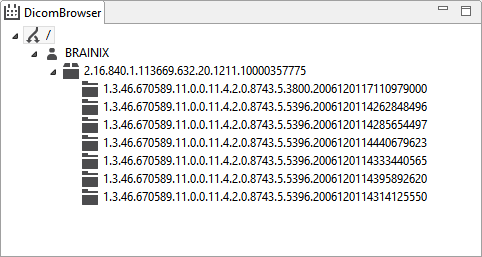
\includegraphics[angle=0,width=9cm]{./img/dicombrowser.png}}
   \caption{Die Baumansicht des DICOM-Browsers mit geladenen Objekten}
  \label{dicombrowser}
  \vspace{0.5cm}
\end{figure}

%\FloatBarrier
%\subsection{Die Baumstruktur} \label{treestructure}
Sowohl die Anzeige, als auch die interne Behandlung der Daten soll so nah wie möglich an den DICOM-Standard angelehnt sein und unabhängig von der Auslieferung\footnote{Unabhängig davon, ob Dateien von der Festplatte geladen oder über das Netzwerk bezogen werden.} der Dateien die Struktur des ER-Modells haben.\\
Ein Baum als Datenstruktur erfüllt die grundlegende Repräsentation mit den verschiedenen Knotentypen aus Patientenname, Studien, Serien und den DICOM-Objekten.\\
Dadurch ergibt sich mit der Wurzel eine Höhe von
\begin{equation}
h = max(4)
\label{baumheight}
\end{equation}
und folgende konkrete Höhen der Knotentypen.
\begin{equation}
h_{Root} = 0 \qquad
h_{Patienenname} = 1 \qquad 
h_{Study} = 2 \qquad
h_{Series} = 3 \qquad
h_{Oject} = 4
\label{heights}
\end{equation}

Der minimale Baum besteht nur aus der Wurzel und hat die Höhe $h_{min} = 0$. Nach der Multiplizität des Modells aus Abschnitt \ref{grundlagen:iod} hat der Baum, sobald ein Patientenname eingefügt wird, eine minimale Höhe von $h_{min} = 3$, da Patientenname und Study jeweils mindestens ein Kindelement enthalten. Die Breite des Baums ist unbestimmt, da Knoten eine beliebige Anzahl an Kindern besitzen können. Abbildung \ref{treeexample} zeigt einen Baum, wie er in der Anwendung repräsentiert werden könnte. Der Baum enthält alle Knotentypen von \textit{Patientname} bis \textit{Object}-Ebene.\\
Zwei Klassen des Quelltextes liefern die Basis des Baums:

\begin{itemize}
\item \textbf{DicomTreeRepository}\\
	  Diese Klasse repräsentiert den Baum. Sie enthält den Wurzelknoten, und einige graphentypische Operationen. Der Baum kann nach Knoten durchsucht werden und hat eine Funktion zum Einfügen neuer Knoten. Eine Löschfunktion wurde nicht implementiert, da der Baum nicht vom Benutzer manipuliert werden soll. Das Einfügen soll nur zum initialen Einlesen aufgerufen werden.
\item \textbf{ADicomTreeItem}\\
	  \textit{ADicomTreeItem} bilden die Knoten des Baumes. Jede Instanz besitzt eine Identifikationsnummer und kennt sowohl das Elternelement, als auch die Kindknoten. 
\end{itemize}

\tikzstyle{every node}=[draw=black,thick,anchor=south, align=center]
%\tikzstyle{selected}=[draw=red,fill=red!30]
\tikzstyle{optional}=[dashed,fill=gray!50]
\begin{figure}[htbp]
\centering
\caption{Beispielhafte Darstellung eines Baumes mit $h = 4$ in der Implementierung}
\label{treeexample}
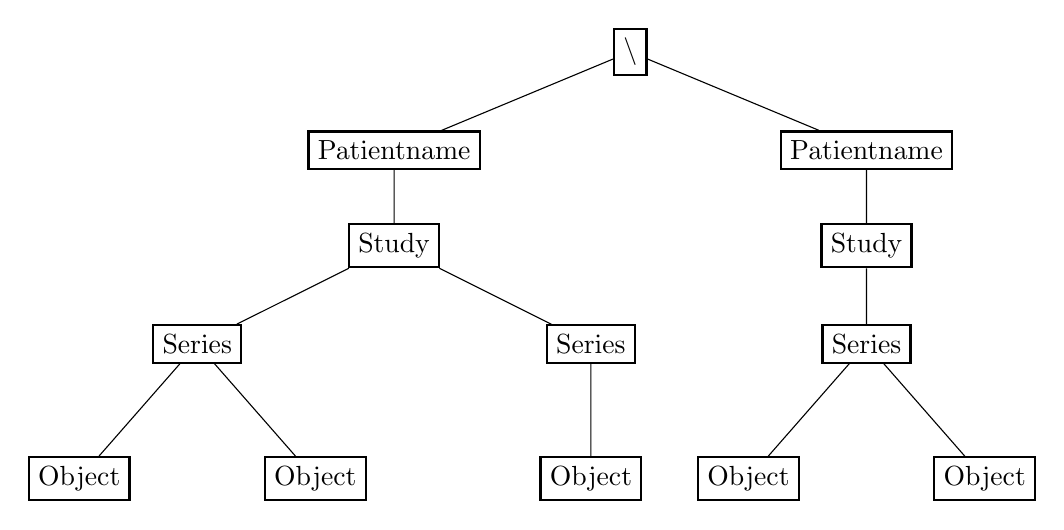
\begin{tikzpicture}[level distance=1.5cm,
  level 1/.style={sibling distance=6cm},
  level 2/.style={sibling distance=5cm},
  level 4/.style={sibling distance = 3cm, level distance = 2cm},
   level 5/.style={sibling distance=1cm},]
  \node {$\backslash$}
    child { node{Patientname}
      child { node{Study}
        child {node{Series}
        	child {node{Object}}
        	child {node{Object}}
        }
        child {node{Series}
          child {node{Object}}
        }
      }
    }
    child { node{Patientname}
    	child{ node{Study}
    	  child{ node{Series}
    	  	child {node{Object}}
    	  	child {node{Object}}
    	  }
    	}
    };
\end{tikzpicture}
\end{figure}

Da nun die Datenstruktur bestimmt ist, fehlt das Vorgehen zur Sortierung der Daten. Abbildung \ref{filesystemrep} in Abschnitt \ref{grundlagen:dicom} zeigt eine mögliche Dateistruktur. Das liefert allerdings keine Sicherheit, dass die Dateien immer vorsortiert zur Verfügung stehen. SLiegen alle DICOM-Dateien in einem Ordner, wäre eine Einteilung in Patienten und Serien etc. nicht mehr möglich.\\
Wie bereits in Abschnitt \ref{grundlagen:dicom} beschrieben besitzt jeder Patient, jede Studie und jede Serie eine eigene eindeutige Identifikationsnummer(UID), die eine modellgerechte Sortierung ermöglicht. Die Tags, die diese UIDs enthalten sind \textit{Patient ID}, \textit{Study Instace UID}, \textit{Series Instance UID} und \textit{SOP Instance UID}.\\
Jede Datei repräsentiert ein Blatt im Baum und somit ein DICOM-Objekt. Dadurch muss die abstrakte Klasse ADicomObjekt aus der Architekturbeschreibung aus Kapitel \ref{architecture} Abschnitt \ref{adapter_dependencies} angepasst werden und erweitert die abstrakte Superklasse ADicomTreeItem. Somit erben alle DICOM-Objekte die Eigenschaften eines Knoten im Baum. Zur weiteren Klassifizierung der Knoten werden die Klassen \textit{DicomPatientItem}, \textit{DicomStudyItem} und \textit{DicomSeriesItem}, die alle von \textit{ADicomTreeItem} erben, eingesetzt.
Bei der Instantiierung des DICOM-Objekts wird direkt die UID über \textit{SOP Instance UID} zugewiesen. Als nächster Schritt wird aus dem DICOM-Objekt der Pfad von der Wurzel zum Objekt ermittelt. Dazu werden \textit{Patient ID}, \textit{Study Instace UID} und \textit{Series Instance UID} des Objekts ausgelesen. Nun wird der Baum nach den entsprechenden Objekten und den UIDs durchsucht. Sind diese nicht vorhanden, wird das zugehörige Objekt erzeugt und in den Baum eingefügt, bis letztendlich das DICOM-Objekt als Blatt eingehängt werden kann.\\
Mittels dieser Sortierung entsprechen die Elemente im DicomBrowser der Darstellung des ER-Modells.

\FloatBarrier
\section{Repräsentation der Pixeldaten}

Ganzzahlige Datentypen in Java (\textit{byte}, \textit{short}, \textit{int}, \textit{long}) werden im Zweierkomplement kodiert\cite[S.106]{java:insel}]. Dadurch sind nur Werte im Bereich von $[-2^{BIT-1}, 2^{BIT-1}-1]$. Das entspricht beim Datentyp \textit{short} dem Intervall von $[-2^{15}, 2^{15}-1] \rightarrow [-32768, 32767]$.\\
Medizinische Grauwertbilder besitzen meist eine Tiefe von 8-, 12- und 16-Bit. Zusätzlich bestimmt der DICOM-Tag \textit{PixelRepresentation}, ob Pixelwerte vorzeichenbehaftet sind. Durch diese variablen Eigenschaften entstehen unterschiedliche Bildtypen. Aus dem Abschnitt \ref{grey_images} wird deutlich, dass Grauwertbilder mit einer Tiefe von 16-Bit den Bereich von $[0,65535]$ abdecken. Dadurch entsteht eine Diskrepanz zwischen dem 16-Bit Java Datentyp \textit{short} und den Grauwerten. Die Pixelwerte können vom Typ \textit{short} nicht aufgenommen werden. Das gleiche Missverhältnis entsteht bei einer Tiefe von 8-Bit. Wie in Tabelle \ref{java:datentypen} zu sehen, fasst der Datentyp \textit{byte} maximal einen Wert von 127 während der größte Pixelwert 255 entspricht. Daraus folgt, dass Grauwertbilder ohne vorzeichenbehaftete Werte (Unsigned) mit dem nächsthöheren Datentyp repräsentiert werden.

\begin{table}
    \begin{tabularx}{\textwidth}{|X|X|X|X|}
    \toprule
    \hline
    \textbf{Datentyp}         & \textbf{MIN}    & \textbf{MAX}& \textbf{Unsigned} \\ \hline
    byte 		 			  & -128					& 127 		  & 0 - 255\\ \hline
    short 		 			  & -32768				& 32767 		  	  & 	0 - 65535\\ \hline
    int						  & -2147483648		& 2147483647 		  & 0 - 4294967295\\ \hline
    long 				      & \tiny{-9223372036854775808}			& \tiny{9223372036854775807} 		  & \tiny{0 - 18446744073709551615}\\ \hline

    \bottomrule
    \end{tabularx}
    \caption {Ganzzahlige Datentypen in Java}
    \label{java:datentypen}
\end{table}

\begin{table}
    \begin{tabularx}{\textwidth}{|p{5cm}|X|X|X|X|}
    \toprule
    \hline
    \textbf{Klassenname}         & \textbf{Pixeltyp Code}    & \textbf{Bittiefe Code}& \textbf{Bittiefe DICOM-Objekt} & \textbf{Vorzeichen} \\ \hline
    UnsignedByteImage 		 	& short					& 16 		  & 8 & \O \\ \hline
    ShortImage 		 			  & short				& 16 		  	  & 	16 & ja\\ \hline
    UnsignedShortImage						  & int		& 32 		  & 16 & \O \\ \hline
    IntegerImage (Farbbild)				      & int		& 32, 8-Bit je Kanal		  & 32, 8-Bit je Kanal & \O \\ \hline

    \bottomrule
    \end{tabularx}
    \caption {Von jMediKit implementierte Bildtypen}
    \label{java:bildtypen}
\end{table}

Tabelle \ref{java:bildtypen} zeigt eine Darstellung der implementierten Bildtypen und die zugehörigen Datentypen der Pixel im Quelltext. Haben die Pixeldaten eines DICOM-Objekts eine Tiefe von 8-Bit und sind nicht vorzeichenbehaftet, wird zur Repräsentation in der Implementierung ein Array des Typs \textit{short} verwendet, um alle Werte aufnehmen zu können.\\
Der Datentyp \textit{int} könnte alle Pixelwerte eines DICOM-Objekts aufnehmen. So liegt es nahe, dass Integer durchgehend als Datentyp verwendet wird. Arbeitet man allerdings mit 8-Bittiefe ohne Vorzeichen, wird der Speicherbedarf von 16 auf 32 Bit pro Pixel verdoppelt. Daher ist es sinnvoll die Bildtypen zu kategorisieren.

\FloatBarrier
\section{Räumliche Sortierung der Bilddaten}

Beim Erstellen des Baums aus Abschnitt \ref{treestructure} wird rekursiv das Verzeichnis durchlaufen und nach lesbaren DICOM-Objekten gesucht. Ist die Suche erfolgreich, wird das Objekt dem Baum hinzugefügt. Hierbei kann das Problem auftreten, dass Dateien in der falschen Reihenfolge importiert werden. So kann es passieren, dass ein Importvorgang abhängig vom Dateinamen Objekte dem Baum hinzufügt. Die räumliche Reihenfolge der einzelnen Schichten entspricht allerdings keineswegs dem Dateinamen\footnote{Je nach Sortierung innerhalb des Betriebssystems könnte ein Import auch nach dem Änderungsdatum erfolgen} oder anderen dateibezogenen Reihenfolgen. Dadurch wird, wie schon bei der Sortierung nach dem ER-Modell, eine Methode benötigt, mittels DICOM-Tags die korrekte Reihenfolge der Bilddaten herzustellen.\\
Der Standard verfügt über mehrere Tags, welche die richtige Reihenfolge andeuten. \textit{Instance Number} ist nach dem Standard \cite[C.7.6.1]{dicom:iod} eine Nummer, die ein Bild identifiziert. Während der Entwicklung entsprach dieser Wert der Testbilder der dargestellten Reihenfolge, jedoch ist keine Information enthalten ob diese der tatsächlichen Reihenfolge im Raum entspricht. So könnte der Wert für die Aufnahmenreihenfolge oder andere konsekutive auf- oder absteigende Folgen stehen. Dadurch ist \textit{Instance Number} nur bedingt geeignet.\\
Ein Tag, der räumliche Informationen enthält ist \textit{Slice Location}. Nach dem Standard \cite[C.7.6.2]{dicom:iod} ist dieser Wert die relative Position der Bildebene in mm. Es ist allerdings keine Information enthalten, ob die Sortierung in steigender oder fallender Reihenfolge erfolgt. Da der Tag zusätzlich nur optional vorhanden ist, kann eine Nutzung zur Bestimmung der Anordnung ausgeschlossen werden.

\begin{figure*}[htb]
%\subfigure[Keypoints]{\includegraphics[width=0.49\textwidth]{./img/basmati_keypoints.png}}\hfill
\centering
\fbox{
\subfigure[Darstellung der beiden Richtungsvektoren der Bildebene und zugehörige Normale $\vec{r} \times \vec{c}$]{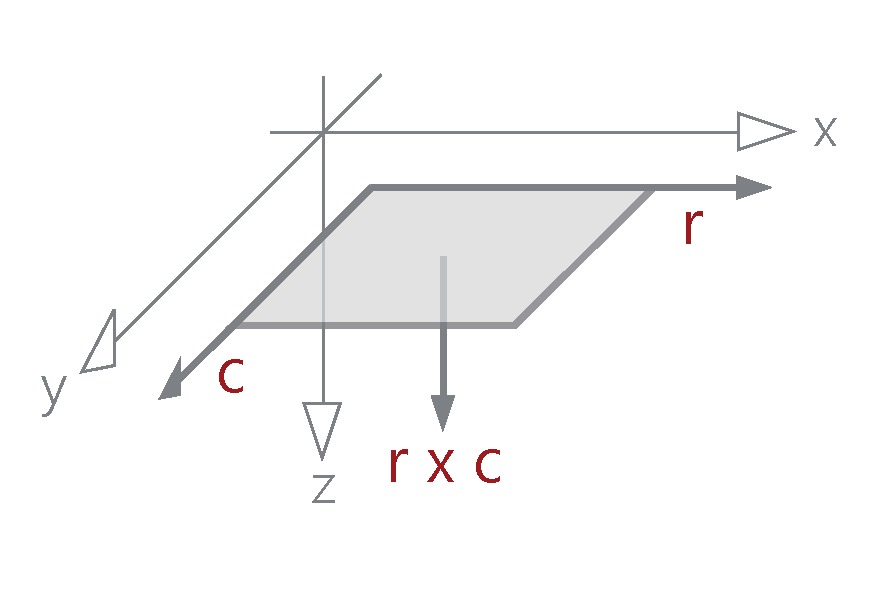
\includegraphics[width=5cm]{./img/normalenvektor.pdf} \label{sort:single}}
\subfigure[Schichten entlang der Normalen $\vec{r} \times \vec{c}$]{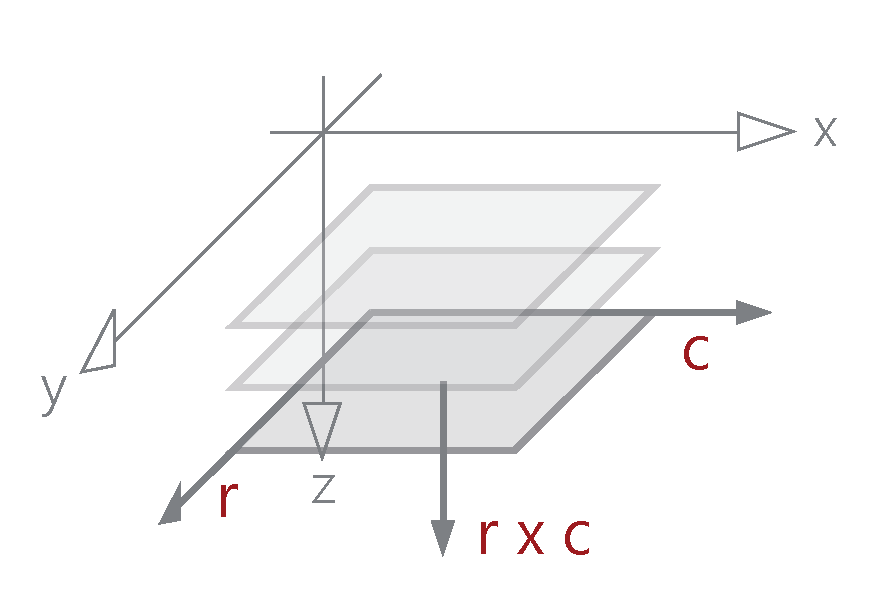
\includegraphics[width=5cm]{./img/normalenvektorstack.pdf} \label{sort:stack}}
\subfigure[Sortierung erfolgt durch Bestimmung der dominanten Achse]{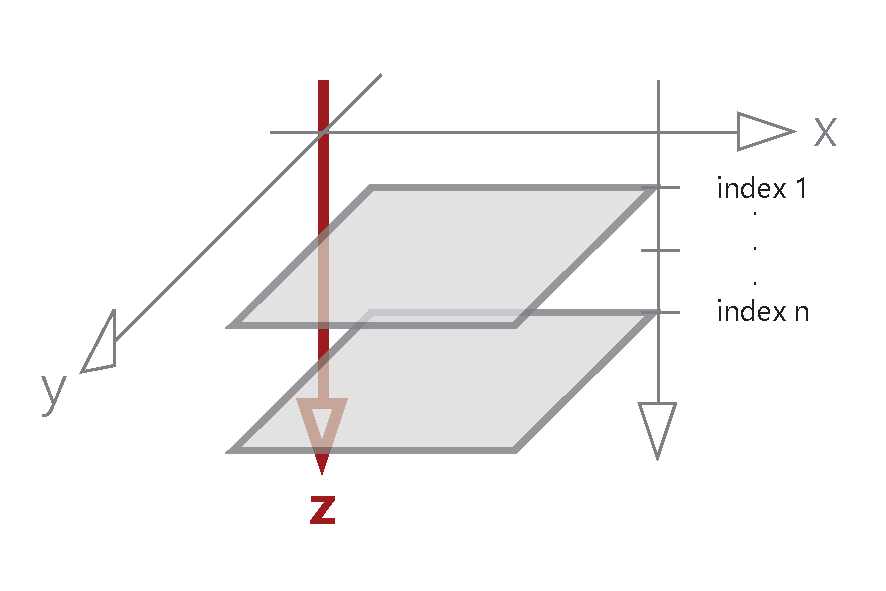
\includegraphics[width=5cm]{./img/dominantindex.pdf} \label{sort:dominant}}
}
\caption{Räumliche Sortierung der DICOM-Objekte}
\label{sort}
\end{figure*}

In der Mailingliste des Insight Segmentation and Registration Toolkits \cite{itk:mail} wird eine Berechnung über die Attribute \textit{Image Position} und \textit{Image Orientation} vorgeschlagen.
\textit{Image Position} enthält die $x$, $y$ und $z$ Koordinate in mm und \textit{Image Orientation} den Richtungskosinus\footnote{Ein Richtungskosinus beschreibt die Winkel des Vektors zu den drei Koordinatenachsen} der ersten Reihe und Spalte des Bildes in Abhängigkeit des Patienten. Diese beiden Richtungsvektoren spannen die Bildebene auf und müssen nach \cite[C.7.6.2.1.1]{dicom:iod} orthogonal zueinander sein.\\
Die Abbildungen in \ref{sort} zeigen das Koordinatensystem des Patienten als rechtshändiges System\cite[S.419]{dicom:iod}. Dieses ist um 180 Grad um die x-Achse gedreht. In Abbildung \ref{sort:single} ist die Bildebene sowie die beiden Richtungsvektoren $\vec{c}$ der ersten Spalte und $\vec{r}$ der ersten Reihe dargestellt. Mit Hilfe des Kreuzproduktes lässt sich nun die Normale der Ebene bestimmen. Die räumliche Anordnung der Schichten erfolgt entlang des Normalenvektors $\vec{r} \times \vec{c}$ (Abbildung \ref{sort:stack}). Die Richtungsvektoren könnten folgende Darstellung besitzen:

\begin{equation}
%\vec{r}=\left(\begin{array}{c} 1 \\ 0 \end{array}\right) \qquad
\vec{r}=\left(\begin{array}{c} 1 \\ 0 \\ 0 \end{array}\right) \qquad
\vec{c}=\left(\begin{array}{c} 0 \\ 1 \\ 0 \end{array}\right) \qquad
\vec{n}=\vec{r}\times\vec{c}=\left(\begin{array}{c} 0 \\ 0 \\ 1 \end{array}\right) \qquad
\vspace{0.5cm}
\label{example_vector}
\end{equation}

Nachdem die Normale $\vec{n}$ der Ebene bestimmt ist, muss der dominante Anteil des Vektors ermittelt werden. Dazu wird der maximale Betrag aus den Elementen von $ \vec{n}$ mit $|n_x|, |n_y|, |n_z|$ berechnet. Somit erhält man die Achse an der die Schichten angeordnet sind. Im Beispiel \ref{example_vector} und Abbildung \ref{sort:dominant} erfolgt die Anordnung entlang der z-Achse, da $n_z$ den dominanten Anteil von $\vec{n}$ darstellt. Ist $n_z < 0$ erfolgt die Wuchsrichtung der Schichten entlang des negativen Anteils der z-Achse. Wenn $n_z >= 0$ wachsen die Ebenen in die positive Richtung.\\
Mit Hilfe dieser Kriterien lassen sich die Bilder über den Tag \textit{Image Position} sortieren. Es ist bekannt, welche Achse die Reihenfolge im Raum symbolisiert. Beispiel \ref{example_sort} zeigt drei Vektoren mit möglichen Daten von \textit{ImagePosition}. Ist der dominante Anteil des Vektors kleiner 0, verläuft die Wuchsrichtung negativ und der größte Wert ist das erste Bild der Folge. Ist der dominante Anteil positiv, hat das erste Bild des kleinsten Wert. Da im Beispiel \ref{example_vector} $n_z >= 0$ entspricht die Sortierte Reihenfolge aus Beispiel \ref{example_sort} $\vec{b}\rightarrow\vec{a}\rightarrow\vec{c}$.

\begin{equation}
%\vec{r}=\left(\begin{array}{c} 1 \\ 0 \end{array}\right) \qquad
\vec{a}_{position}=\left(\begin{array}{c} 13.6 \\ 122 \\ 75 \end{array}\right) \qquad
\vec{b}_{position}=\left(\begin{array}{c} 13.7 \\ 121.6 \\ 65 \end{array}\right) \qquad
\vec{c}_{position}=\left(\begin{array}{c} 12.6 \\ 122.1 \\ 85 \end{array}\right) \qquad
\vspace{0.5cm}
\label{example_sort}
\end{equation}

Durch eine Implementierung des Interface \textit{Comparable\textless AImage\textgreater} in \textit{AImage} unter Berücksichtigung dieser Vorgehensweise ist eine einfache und für diesen Zweck ausreichend schnelle Sortierung der Bildebenen mögliche. Somit erfolgt die Anordnung des Baums und der Bilder unabhängig der Dateistruktur.\\
Voraussetzung für diese Umsetzung ist, dass die Bildebenen parallel zu den Koordinatenachsen verlaufen. Bei Bildreihen mit Kurven oder einem schrägen Verlauf kann keine dominante Achse bestimmt werden.

\FloatBarrier
\section{Zeichnen und manipulieren der Bilddaten} \label{drawandmanipulate}

Sowohl die DICOM-Objekte, als auch Bilddaten stehen im Speicher zur Verarbeitung bereit. Dieser Abschnitt befasst sich mit der Visualisierung dieser Daten. Wie aus Kapitel \ref{architecture} Abschnitt \ref{ivp_architecture} bekannt ist, erfolgt die Darstellung der Bilder im \textit{ImageViewPart} der Anwendung. Innerhalb des Parts können bis zu vier \textit{ImageViewComposites } angezeigt werden. Diese dienen vor allem zur Bedienung des enthaltenen \textit{DicomCanvas}. So kann mit Hilfe der Scrollleiste durch den dreidimensionalen Datensatz navigiert, oder Informationen wie das Koordinatensystem angezeigt und versteckt werden. Die tatsächliche Anzeige der Bilddaten findet im Canvas-Element statt. Eine direkte Manipulation der Bilder erfolgt durch die Auswahl eines Werkzeugs.\\
Die Breite und Höhe der Zeichenfläche ist unter anderem abhängig von der Zahl der angezeigten \textit{ImageViewComposites}, der Bildschirmgröße und dessen Auflösung. Je mehr Composites angezeigt werden, desto kleiner wird der Bereich für das \textit{DicomCanvas}. So kann der Fall eintreten, dass die Dimension der Zeichenfläche nicht ausreicht, um ein Bild vollständig anzuzeigen, da das Bild größer als die zur Verfügung stehender Fläche ist. Dadurch muss dem Nutzer eine Möglichkeit gegeben werden, nicht sichtbare Details in den sichtbaren Bereich schieben zu können.\\
Neben dem Verschieben des Bildes gibt es zwei weitere essentielle Werkzeuge zur Manipulation medizinischer Bilddaten. Bei einer Darstellung in 100\% der Bildgröße sind Details nicht immer gut zu erkennen. Dadurch muss eine Skalierung des Bildes möglich sein.
Das zweite Werkzeug übernimmt die Fensterung der Grauwerte. Je nach Struktur oder Gewebe das betrachtet werden soll, müssen die Fensterungswerte individuell zu wählen sein.
Zusätzlich zu den Werkzeugen gibt es drei verschiedene Ansichten, aus denen der Benutzer wählen kann. Damit kann bestimmt werden, welche Ebene der 3D-Bilddaten angezeigt werden soll. Abbildung \ref{layers} zeigt die verschiedenen Optionen. Die einzelnen Ansichten sind die $(x,y)$-Ebene (axial), die $(x,z)$-Ebene (coronal) und die $(y,z)$-Ebene (sagittal).\\
\begin{figure*}[htb]
%\subfigure[Keypoints]{\includegraphics[width=0.49\textwidth]{./img/basmati_keypoints.png}}\hfill
\centering
\fbox{
\subfigure[Axiale Ansicht - $(x,y)$]{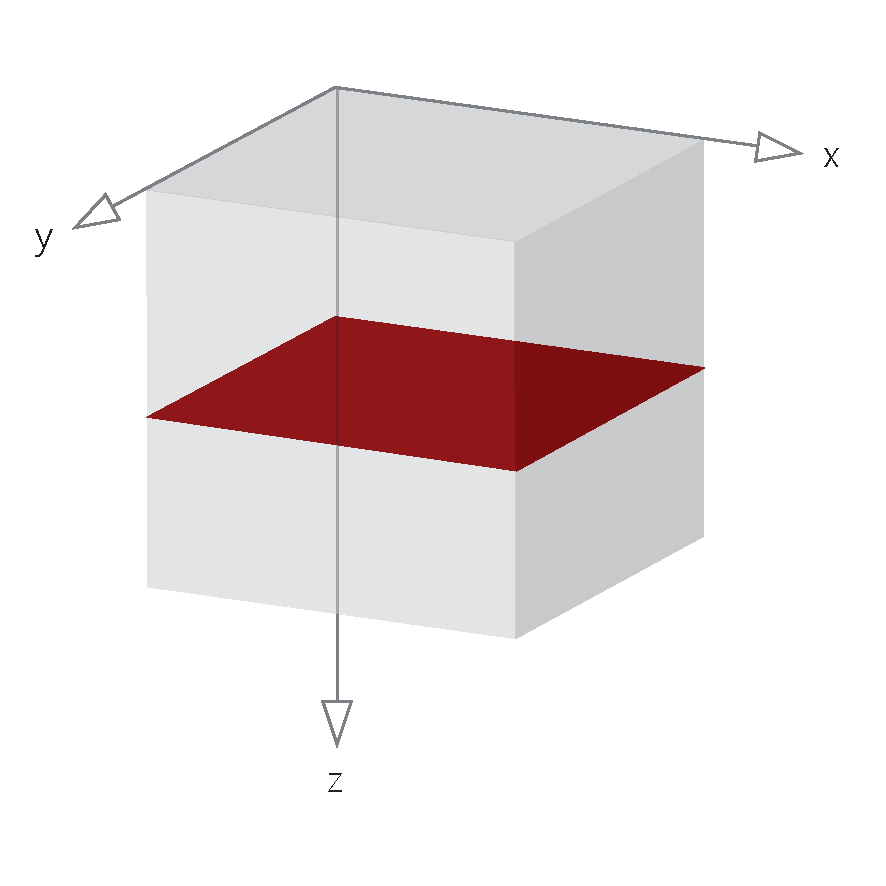
\includegraphics[width=5cm]{./img/axial_xy.pdf} \label{layers:axial}}
\subfigure[Coronale Ansicht - $(x,z)$]{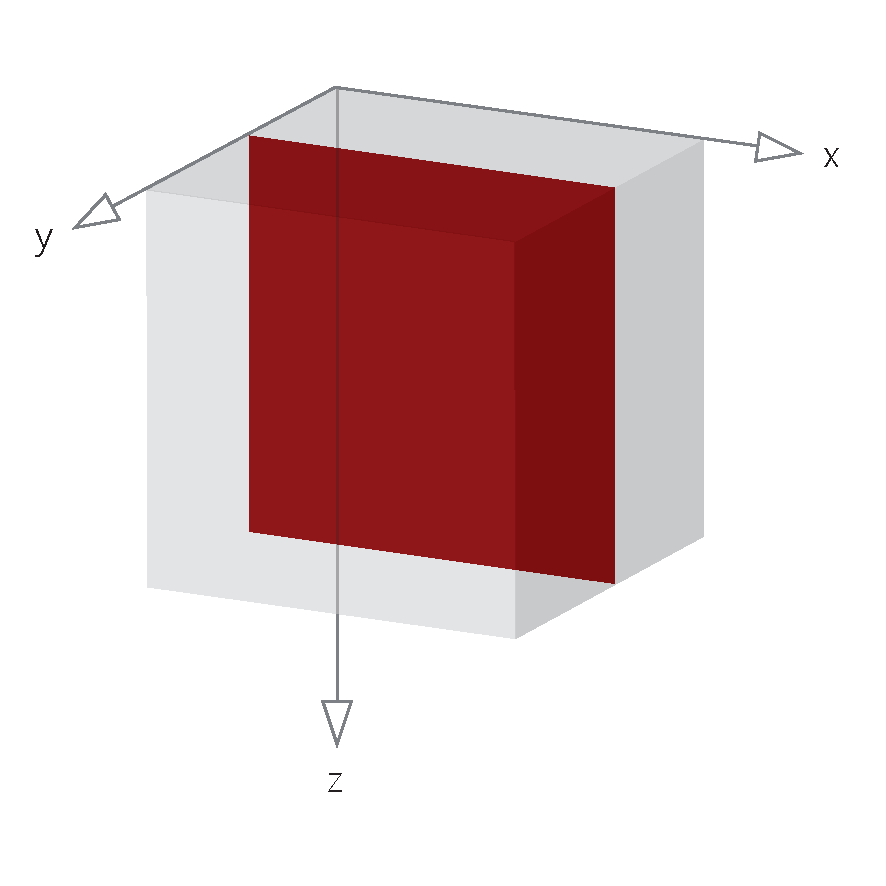
\includegraphics[width=5cm]{./img/coronal_xz.pdf} \label{layers:coronal}}
\subfigure[Sagittale Ansicht - $(y,z)$]{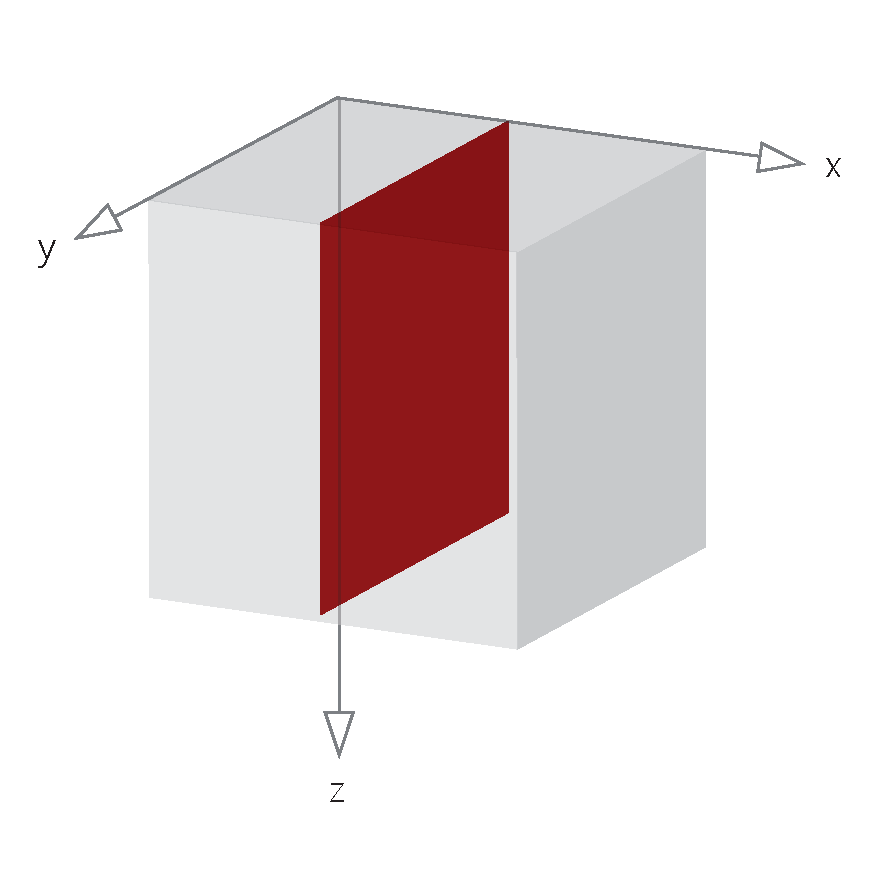
\includegraphics[width=5cm]{./img/sagittal_yz.pdf} \label{layers:sagittal}}
}
\caption{Die verschiedenen Ansichten der Ebenen eines dreidimensionalen Datensatzes}
\label{layers}
\end{figure*}

Die Faktoren DICOM-Objekt, Bedienelemente der Composites, Werkzeuge und die verschiedenen Ansichten der Ebenen beeinflussen maßgeblich den Prozess der Anzeige der Bilddaten. Die Vorgehensweise wird in Abbildung \ref{imageprocess} visualisiert. Der Prozess gliedert sich in sechs zentrale Verarbeitungsblöcke und zwei Einhängepunkte(Hooks) für Werkzeuge.

\begin{figure}[htbp]
  \vspace{0.5cm}
  \centering
  \fbox{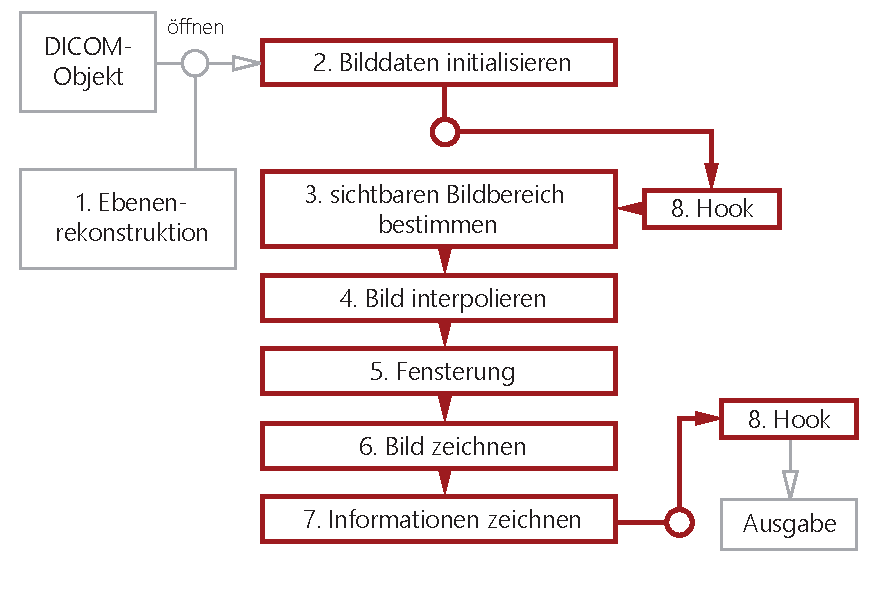
\includegraphics[angle=0,width=10cm]{./img/imageprocess.pdf}}
   \caption{Der Prozess von der Bildauswahl zur Anzeige}
  \label{imageprocess}
  \vspace{0.5cm}
\end{figure}

\begin{enumerate}
\item \textbf{Ebenenrekonstruktion}\\
	Nach Bedarf hat der Anwender die Möglichkeit eine axiale, coronale oder sagittale Ebenendarstellung zu wählen. Wird diese Option angewendet, wird der Bilddatensatz neu berechnet.
\item \textbf{Bilddaten initialisieren}\\
	Abhängig vom gewählten Index der Scrollleiste des \textit{ImageViewComposites} wird das entsprechende Bild aus dem 3D-Datensatz geladen.
\item \textbf{Koordinaten des geladenen Bildes berechnen}\\
	Wird ein Bild auf der Zeichenfläche verschoben, ändern sich die Koordinaten des Bildes. Dieser Block übernimmt die Berechnung, damit die Daten korrekt angezeigt werden.
\item \textbf{Bild interpolieren}\\
	Bei einer Skalierung ändert sich die Bildgröße. Die fehlenden Pixel einer Vergrößerung müssen interpoliert werden.
\item \textbf{Fensterung}\\
	Mit Hilfe der Fensterung werden die Grauwerte entsprechend den Werten von Window Width und Window Center auf den Bereich von 0 - 255 abgebildet.
\item \textbf{Bild zeichnen}\\
	Nachdem alle notwendigen Werte berechnet und die Grauwerte durch die Fensterung bestimmt wurden, kann das Bild auf der Zeichenfläche abgebildet werden.
\item \textbf{Informationen zeichnen}\\
	Der nächste Schritt ist das Zeichnen zusätzlicher Informationen für den Anwender. Hierzu zählen zum Beispiel die Koordinatenachsen oder die Werte zu Window Width und Window Center, Bildgröße sowie die Orientierungslinien.
\item \textbf{Hooks}\\
	Beide Hooks stellen Einhängepunkte für Werkzeuge dar. Das sind abstrakte Funktionen, die von konkreten Werkzeugen implementiert werden. Jeweils vor den Berechnungen und nach Abschluss des Zeichenvorgangs werden diese Funktionen aufgerufen und ausgeführt. So könnten zum Beispiel je nach Werkzeug zusätzliche Informationen eingezeichnet werden.
\end{enumerate}

Die Bereiche der Rekonstruktion, Koordinatenberechnung, Interpolation und das Zeichnen der Informationen werden in den folgenden Abschnitten genauer erläutert. Die Initialisierung und das Zeichnen des Bildes sind einfache Operationen. Die Fensterung entspricht dem Algorithmus \ref{windowing_algo} aus Abschnitt \ref{windowing}.

\FloatBarrier
\subsection{Die Rekonstruktion der Ebenen}

Mit einem dreidimensionalen Datensatz ist es möglich, eine beliebige Ebene durch die Voxel zu legen. Dadurch kann man unter anderem eine dreidimensionale Darstellung berechnen, da die Ebenen aus frei wählbaren Winkeln betrachtet werden können. Im Rahmen der Anwendung dieser Arbeit ist die axiale, coronale und sagittale Darstellung allerdings ausreichend.

\begin{figure*}[htb]
\centering
\fbox{
\subfigure[Rekonstruktion von der axialen zur coronalen Ebene]{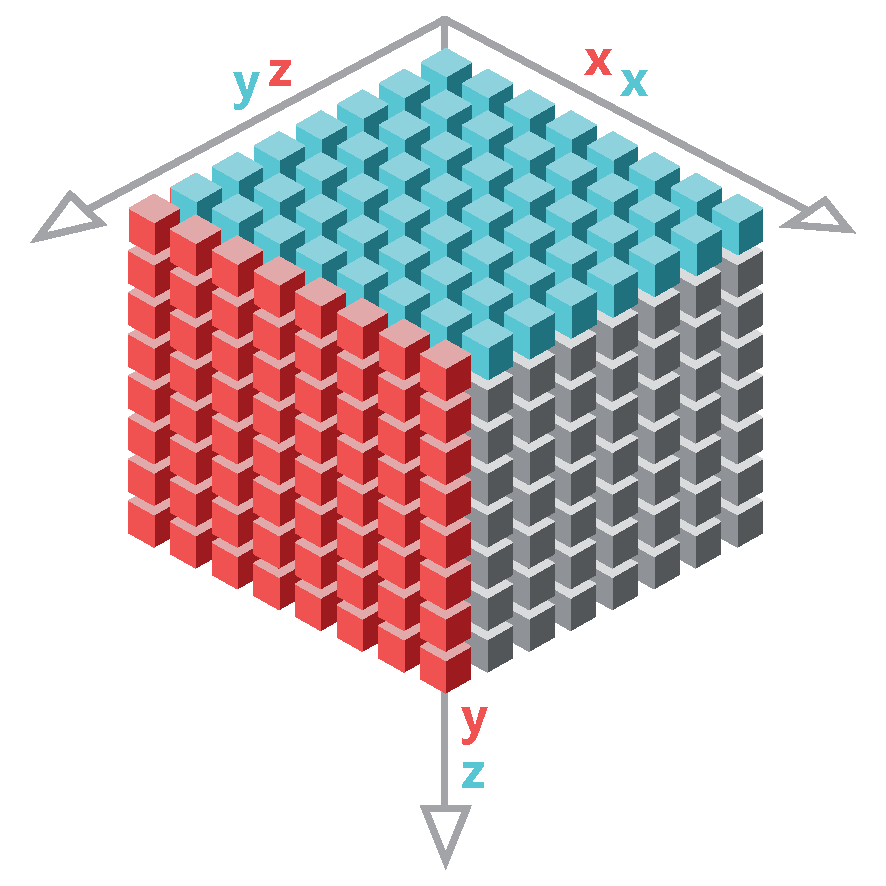
\includegraphics[width=7cm]{./img/axialcoronalmpr.pdf} \label{mpr:ac}}
\subfigure[Rekonstruktion von der axialen zur sagittalen Ebene]{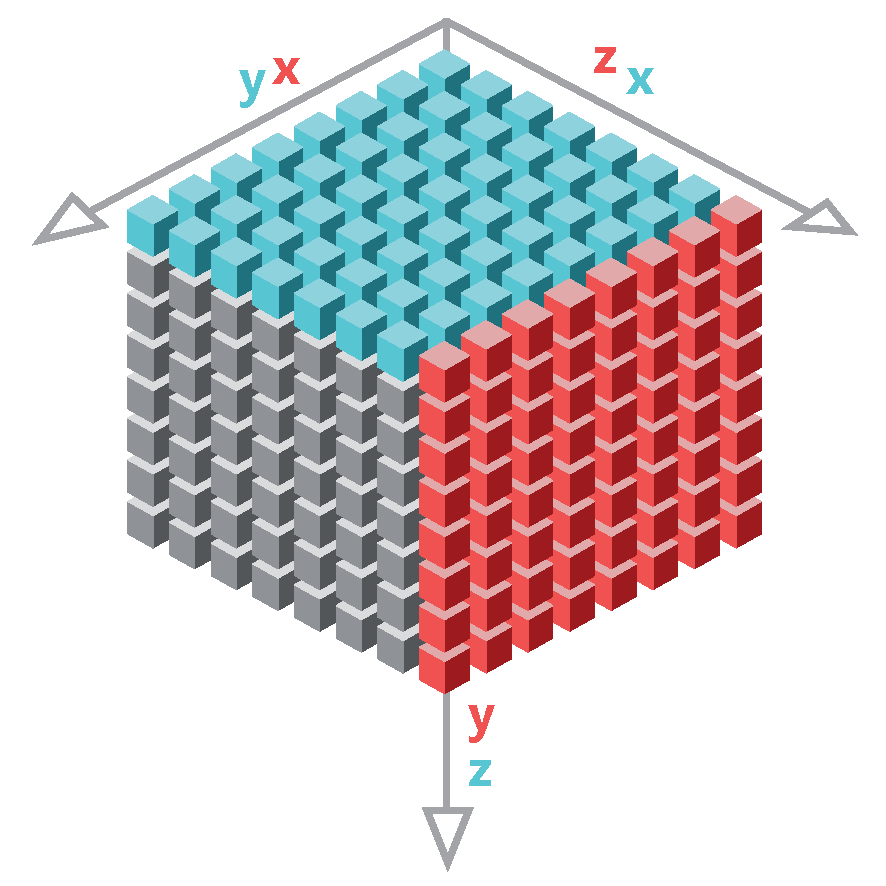
\includegraphics[width=7cm]{./img/axialsagittalmpr.pdf} \label{mpr:as}}
}
\caption{Rekonstruktion der coronalen und sagittalen Ebene}
\label{mpr}
\end{figure*}

Die Abbildungen \ref{mpr} zeigen jeweils die \textit{erste} Bildschicht der axialen Quelldarstellung als blaue und die \textit{letzte} Schicht der Zieldarstellung als rote Voxel. Da die Quell- und Zielebene immer orthogonal zueinander sind, kann auf zeitintensive Berechnungen verzichtet werden. Die neuen Bildebenen können über die Indizes der Pixel der verschiedenen Bilder schnell bestimmt werden. Die Bildgröße der rekonstruierten Ebene ist abhängig von der ursprünglichen Ebenendarstellung. So entspricht, wie Abbildung \ref{mpr:ac} zeigt, die Höhe(y) eines coronalen Bildes der Tiefe(z) einer axialen Darstellung und die coronale Tiefe(z) der axialen Höhe(y). Die Bildbreite bleibt unverändert. Die erste Pixelreihe der Rekonstruktion kann mit den Werten der letzten Reihe der ersten axialen Bildschicht belegt werden. Ein Algorithmus könnte wie folgt implementiert werden:

\begin{algorithm}
\caption{Berechnung der Bildebenen von axialer zu coronaler Darstellung}
\begin{algorithmic}[1] 
\STATE $images \leftarrow input$ - Quellbilder in axialer Darstellung
\STATE $reconstruction \leftarrow output$ - rekonstruierte coronale Bildebenen
\STATE $X_{coronal} \leftarrow X_{axial}$
\STATE $Y_{coronal} \leftarrow Z_{axial}$
\STATE $Z_{coronal} \leftarrow Y_{axial}$

\FORALL{$z \in Z_{coronal}$}
    \FORALL{$y \in Y_{coronal}$}
        \FORALL{$x \in X_{coronal}$}
        	\STATE $i \leftarrow$  get $image(y)$ from $images$ \COMMENT{$y$ entspricht dem $z$-Wert}
        	\STATE $p \leftarrow$ get $pixel(x, z)$ from $i$ \COMMENT{$x$ entspricht dem $x$-Wert und $z$ dem $y$-Wert}
            \STATE set $reconstructedPixel(xy)$ = $p$
        \ENDFOR
    \ENDFOR
\ENDFOR

\end{algorithmic}
\label{mpr_algo}
\end{algorithm}

Nachdem die Bildebenen neu berechnet wurden, muss zusätzlich eine Drehung der Richtungsvektoren im DICOM-Tag \textit{ImageOrientation} vorgenommen werden. Aufgrund der Orthogonalität wird immer in 90$^\circ$-Winkeln um die x-, y- und z-Achsen gedreht. Dadurch wird gewährleistet, dass spätere Berechnungen, wie zum Beispiel die Beschriftung der Koordinatenachsen, korrekt durchgeführt werden können.
Die Drehung erfolgt mit Hilfe der Drehmatrizen. Es wird zuerst um die x-, gefolgt von der y- und z-Achse rotiert.

\begin{figure*}[tbp]
%\subfigure[Keypoints]{\includegraphics[width=0.49\textwidth]{./img/basmati_keypoints.png}}\hfill
\centering
\fbox{
\subfigure[Richtungsvektoren der axialen Bildebene werden um 90$^\circ$ um die x-Achse gedreht]{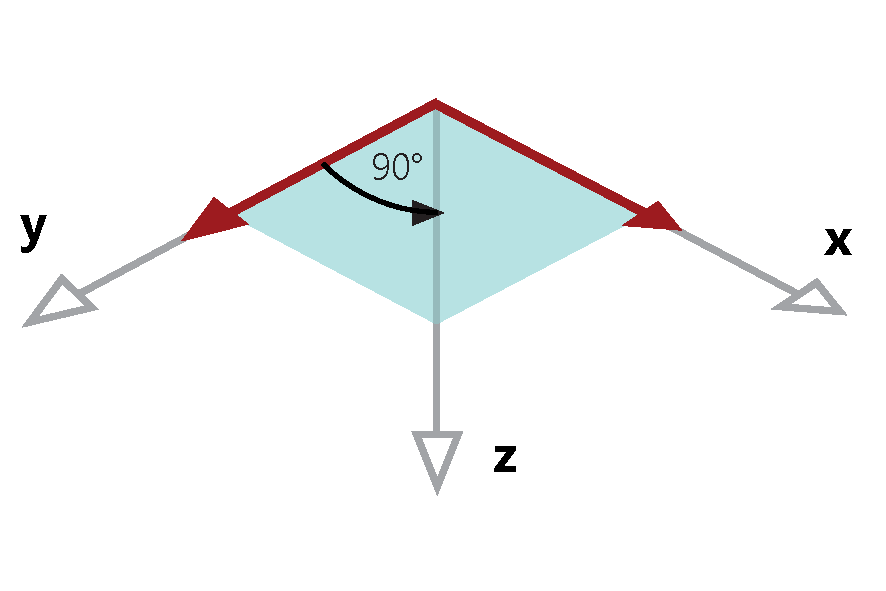
\includegraphics[width=6cm]{./img/rotation.pdf} \label{rota:a}}
\subfigure[Richtungsvektoren in coronaler Ausrichtung]{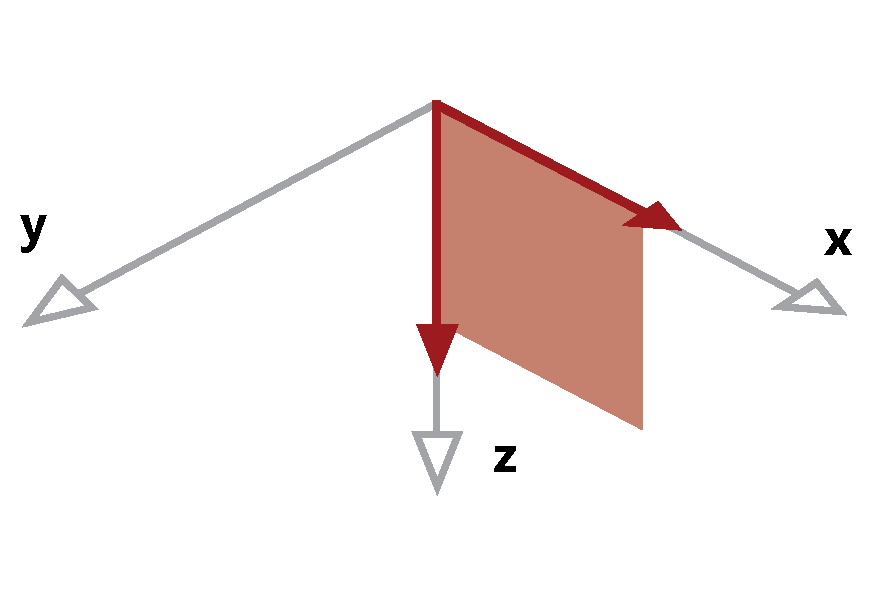
\includegraphics[width=6cm]{./img/rotationc.pdf} \label{rota:c}}
}
\caption{Rotation der Richtungsvektoren von axialer zu coronaler Darstellung}
\label{rota}
\end{figure*}


Die Abbildungen \ref{rota:a} und \ref{rota:c} zeigen den Prozess der Drehung von der axialen in die coronale Ebenendarstellung mit einer Rotation über 90$^\circ$ um die x-Achse.  Folgende Drehmatrix wird zur Berechnung eingesetzt \cite[7.3.2]{nisch:bv}. 

\begin{equation}
R^x=\left(
			\begin{array}{c} 1 \\ 0 \\ 0 \\ 0 \end{array}
			\begin{array}{c} 0 \\ \cos \alpha \\ \sin \alpha \\ 0 \end{array}
			\begin{array}{c} 0 \\ -\sin \alpha \\ \cos \alpha \\ 0 \end{array}
			\begin{array}{c} 0 \\ 0 \\ 0 \\ 1 \end{array}
		\right)
\vspace{0.5cm}
\label{rotation_x}
\end{equation}

Die Rotationsrichtung und die Drehachse ist, wie die rekonstruierten Bilder, abhängig von der Quell- und Zieldarstellung. So könnte eine sagittale Darstellung aus axialen Richtungsvektoren durch eine Drehung um die x-Achse, gefolgt von einer Rotation um die z-Achse berechnet werden.

\FloatBarrier

\subsection{Berechnung der Bildkoordinaten}
Die Werkzeuge zur Translation und Skalierung beeinflussen die Koordinaten des Bildes. Während das Verschieben unproblematisch für die Performance der Anwendung ist, hat die Skalierung, im Besonderen die Vergrößerung, maßgeblichen Einfluss auf die Rechenzeit. Angenommen die Zeichenfläche hat eine Größe von $500 \times 500$ und $250.000$ Pixel und das Bild mit den Maßen $1000 \times 1000$  und $1.000.000$ Pixel die doppelte Größe. Daraus folgt, dass maximal $\frac{1}{4}$ der Pixel des Bildes auf der Zeichenfläche angezeigt werden können. Die sechs Blöcke des Prozesses verarbeiten auch die nicht sichtbaren Anteile des Bildes und verbrauchen dadurch unnötig Rechenzeit. In dem Beispiel bedeutet das einen Mehraufwand von $75\%$. Um diese zusätzliche Rechenzeit einzusparen, darf die Berechnung der Bildkoordinaten nur den aktuell sichtbaren Bereich in die Rechnungen einbeziehen.\\

\begin{figure*}[htb]
%\subfigure[Keypoints]{\includegraphics[width=0.49\textwidth]{./img/basmati_keypoints.png}}\hfill
\centering
\fbox{
\subfigure[Die Koordinaten eines Bildes]{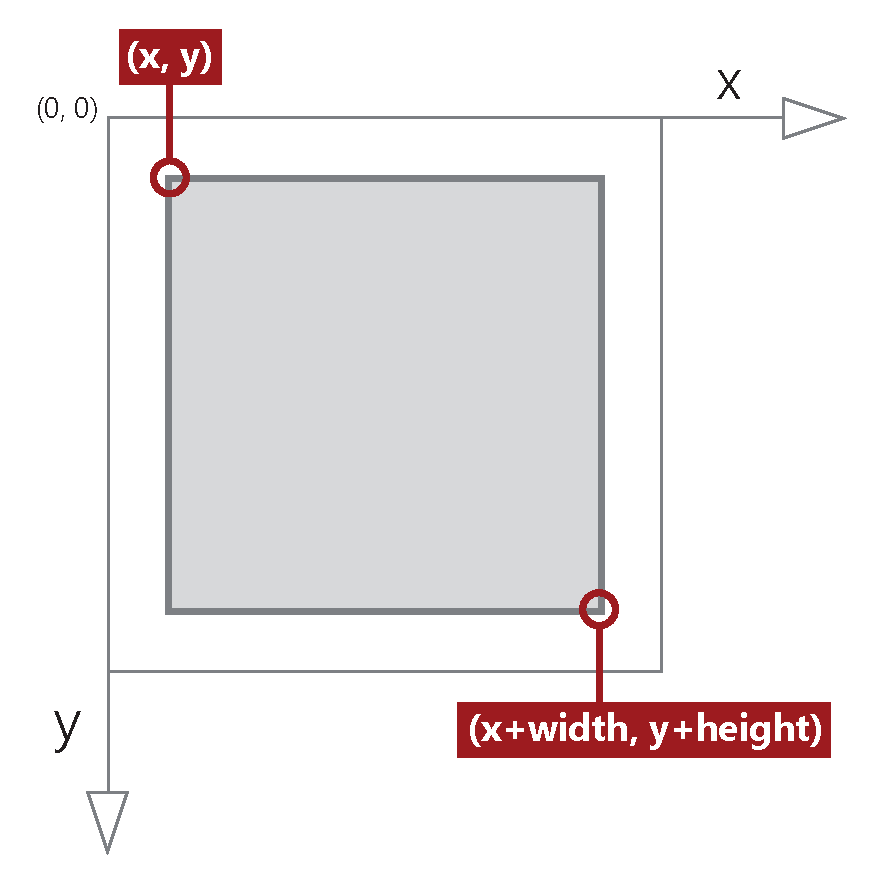
\includegraphics[width=5cm]{./img/bildcoords.pdf} \label{coords:bild}}
\subfigure[Berechnung des sichtbaren Bereichs]{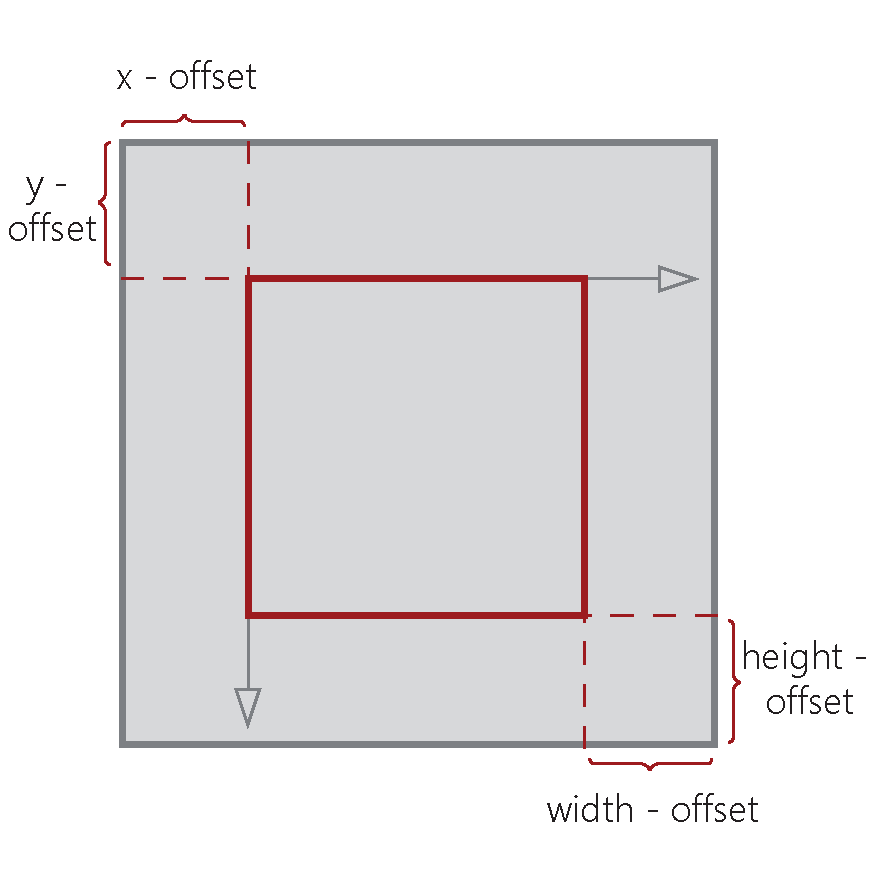
\includegraphics[width=5cm]{./img/offsetcoords.pdf} \label{coords:offset}}
\subfigure[Normalisierte Koordinaten]{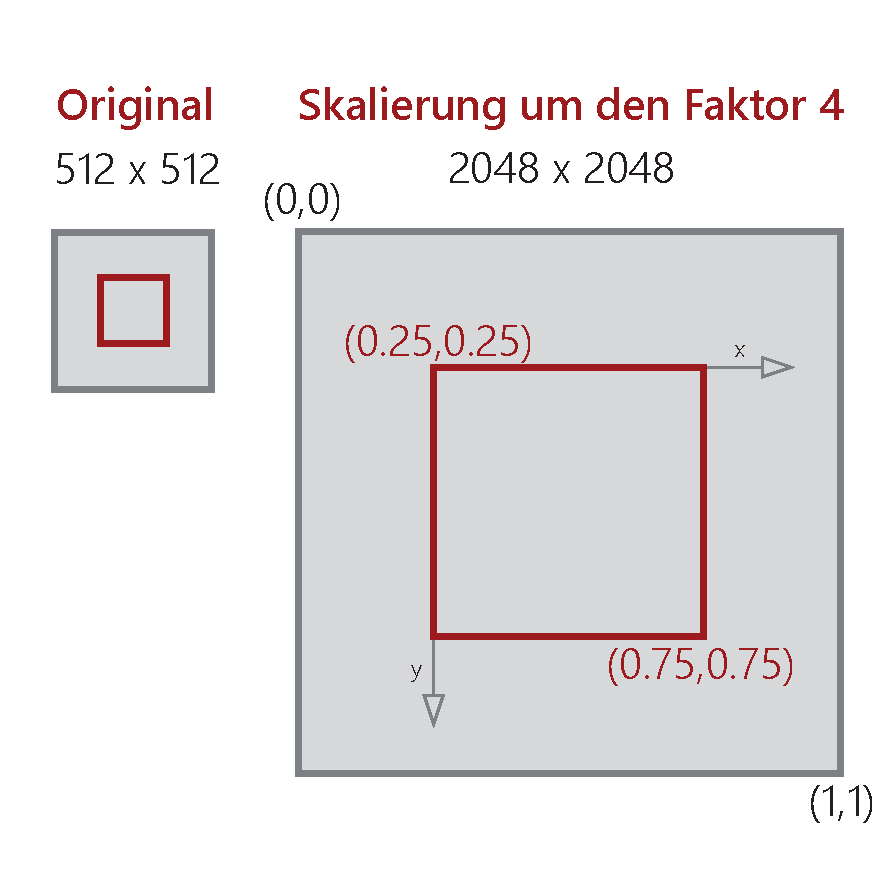
\includegraphics[width=5cm]{./img/bildausschnitt.pdf} \label{coords:normal}}
}
\caption{Berechnung der Position und Koordinaten. Die graue Fläche symbolisiert das Bild und der rote Rahmen stellt den sichtbaren Bildausschnitt dar.}
\label{coords}
\end{figure*}

Wie Abbildung \ref{coords:bild} zeigt, bestimmt \textit{DicomCanvas} das Koordinatensystem mit der linken oberen Ecke als Ursprung. Die Position der Bilder wird durch vier Parameter bestimmt. Die Koordinaten $(x, y)$ legen den Ursprung des Bildes fest und $(widht, height)$ bestimmen mit Breite und Höhe die Dimension. Die tatsächlichen Koordinaten des Bildes sind dadurch $(x, y)$ und $(x+width, y+height)$. Liegen diese vier Parameter außerhalb der Zeichenfläche wie in Abbildung \ref{coords:offset}, muss der Abstand (offset) von x, y, width und height zum Canvas berechnet werden.\\
Das \textit{DicomCanvas} speichert nur das Originalbild und den aktuell sichtbaren Bildausschnitt. Da bei skalierten Bildern nur die Dimension und nicht die Pixeldaten hinterlegt sind, muss der sichtbare Bereich aus dem Original interpoliert werden. Um die richtigen Pixelwerte zu finden, wird mit normalisierten Koordinaten zwischen den Werten $(0, 0)$ für $(x,y)$ und $(1, 1)$ für $(x+width, y+height)$ gearbeitet. Abbildung \ref{coords:normal} zeigt ein Bild mit der Dimension $512 \times 512$, das um den Faktor vier auf $2048\times2048$ vergrößert wurde. Der sichtbare Bildausschnitt erstreckt sich von $(512, 512)$ bis $(1536, 1536)$. Das entspricht dem Bereich von $(128, 128)$ bis $(384, 384)$ im Originalbild. Mit Hilfe der normalisierten Koordinaten lassen sich die Bildbereiche bei gleichem Seitenverhältnis von Original und skaliertem Bild unabhängig von der Größe bestimmen. Für den Bildausschnitt im Beispiel entspricht der Bereich in normalisierter Darstellung $(0.25, 0.25)$ für $(x,y)$ und $(0.75, 0.75)$ für $(width, height)$. Mit gegebenen Pixelwerten lassen sich die normalisierten Koordinaten wie folgt bestimmen.

\begin{equation}
 x_{norm} = \frac{x}{width} \qquad
 y_{norm} = \frac{y}{height}
\end{equation}

Entsprechend dieser Gleichung erfolgt die Berechnung der Indizes von x und y.

\begin{equation}
 x = x_{norm} \cdot width \qquad
 y = y_{norm} \cdot height
\end{equation}

Mit diesen Hilfsmitteln lässt sich nun der obere linke und untere rechte Abstand des Bildes zur Zeichenfläche bestimmen. Zuerst wird geprüft ob $x$ und/oder $y$ einen Wert \textless 0 haben. Ist dies der Fall folgt daraus, dass das Bild aus der oberen und/oder linken Ecke der Zeichenfläche ragt. Die normalisierten Koordinaten lassen sich mit der Formel

\begin{equation}
 x_{norm} = \frac{|x|}{width} \qquad
 y_{norm} = \frac{|y|}{height}
\end{equation}

ermitteln. $x$ und $y$ sind der Abstand vom Ursprung des Koordinatensystems zum Ursprung des Bildes und somit nicht Teil des sichtbaren Bildausschnittes. Der Betrag ist notwendig, da nur Werte zwischen 0 und 1 als normalisierte Koordinaten akzeptiert werden.\\
Angenommen es existiert das Bild aus dem Beispiel in Abbildung \ref{coords:normal} mit den Koordinaten $(-512, -512)$, $(1536, 1536)$ und einer Dimension $(width, height)$ von $()2048, 2048)$ sowie eine Zeichenfläche mit der Dimension $(0, 0)$ und $(1024, 1024)$, dann ergeben sich daraus folgende normalisierte Koordinaten:

\begin{equation}
 x_{norm} = \frac{|-512|}{2048} = 0.25\qquad
 y_{norm} = \frac{|-512|}{2048} = 0.25
\end{equation}

Sind $x$ und/oder $y$ \textgreater= 0 folgt daraus, dass die obere linke Ecke des Bildes vollständig zu sehen ist. Das entspricht dem normalisierten Werten $(0, 0)$.\\
Der nächste Schritt ist die Prüfung der unteren Rechten Ecke. Bevor die Koordinaten bestimmt werden, muss der Abstand berechnet werden, da dieser nicht wie bei $x$ und $y$ abgelesen werden kann. Durch Subtraktion der Bildkoordinaten $(x+width, y+height)$ von der Zeichenfläche erhält man den Abstand zwischen Bild und Canvas.

\begin{equation}
 offset_{width} = x + width - width_{Canvas}\qquad
 offset_{height} = y + height - height_{Canvas}
\end{equation}

Subtrahiert man den Abstand von der Bilddimension erhält man die tatsächlichen Koordinaten, die noch im sichtbaren Bereich der Zeichenfläche liegen. Damit lassen sich die normalisierten Koordinaten berechnen.

\begin{equation}
 x_{norm} = \frac{width - offset_{width}}{width} \qquad
 y_{norm} = \frac{height - offset_{height}}{height}
\end{equation}

Für die Daten aus dem Beispiel ergeben sich folgende Werte:
\begin{equation}
 offset_{width} = -512 + 2048 -1024 = 512\qquad
 offset_{height} = -512 + 2048 -1024 = 512
\end{equation}

\begin{equation}
 x_{norm} = \frac{2048 - 512}{2048} = 0.75\qquad
 y_{norm} = \frac{2048 - 512}{2048} = 0.75
\end{equation}

Mit den berechneten Werten der normalisierten Koordinaten $(0.25, 0.25)$ und $(0.75, 0.75)$ lässt sich der zu interpolierende Bereich aus dem Originalbild bestimmen.

\begin{equation}
 x_1 = 0.25 \cdot 512 =  128\qquad
 y_1 = 0.25 \cdot 512 =  128
\end{equation}

\begin{equation}
 x_2 = 0.75 \cdot 512 =  384\qquad
 y_2 = 0.75 \cdot 512 =  384
\end{equation}

\subsection{Bilineare Interpolation}

Es können verschiedene Interpolationsmethoden eingesetzt werden, um das Bild oder einen Bildausschnitt zu vergrößern oder zu verkleinern. Die Abbildungen \ref{interpolation} zeigen die Ergebnisse einer Nearest Neighbor, biliniearer und bikubischen Interpolation. Das Nearest Neighbor Verfahren stellt die schnellste Interpolationsmethode dar, liefert allerdings auch gleichzeitig die schlechtesten Ergebnisse. In Abbildung \ref{interpolation:nn} erkennt man deutlich die Stufenbildung im Bild.\\
Bessere Ergebnisse liefert die bilineare Interpolation bei einer moderaten Laufzeit. Eine nochmals verbesserte Darstellung kann durch die bikubische Interpolation erreicht werden, benötigt allerdings den größten Rechenaufwand. Die bilinieare Methode liefert einen guten Kompromiss aus Qualität des skalierten Bildes und benötigte Rechenzeit.

\begin{figure*}[htb]
%\subfigure[Keypoints]{\includegraphics[width=0.49\textwidth]{./img/basmati_keypoints.png}}\hfill
\centering
\fbox{
\subfigure[Der rote Rahmen stellt den vergrößerten Ausschnitt aus den Abbildungen \ref{interpolation:nn}, \ref{interpolation:bilinear} und \ref{interpolation:bicubic} dar.]{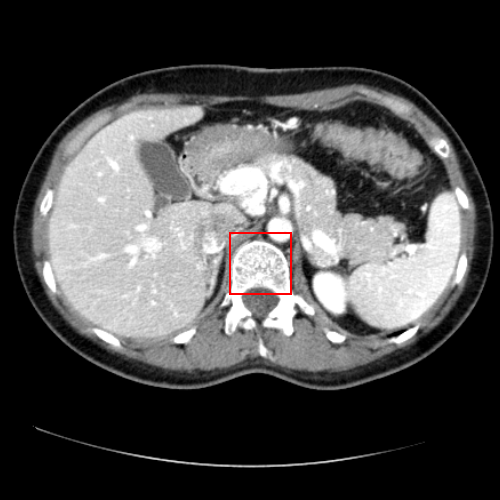
\includegraphics[width=3.6cm]{./img/interpol_src.png} \label{interpolation:src}}
\subfigure[Nearest Neighbor Interpolation]{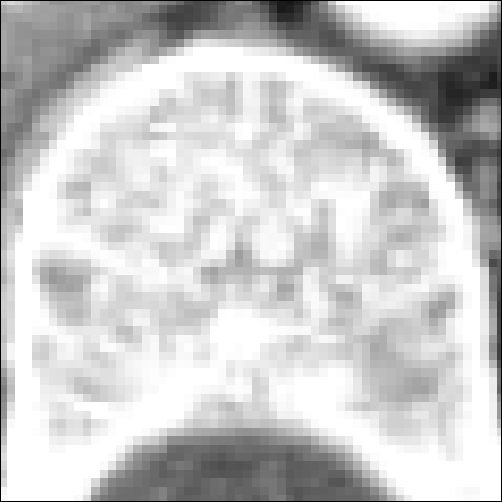
\includegraphics[width=3.6cm]{./img/nn_interpol.png} \label{interpolation:nn}}
\subfigure[Bilineare Interpolation]{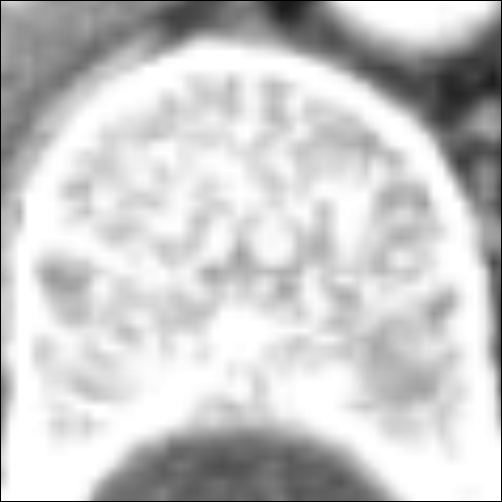
\includegraphics[width=3.6cm]{./img/bilin.png} \label{interpolation:bilinear}}
\subfigure[Bikubische Interpolation]{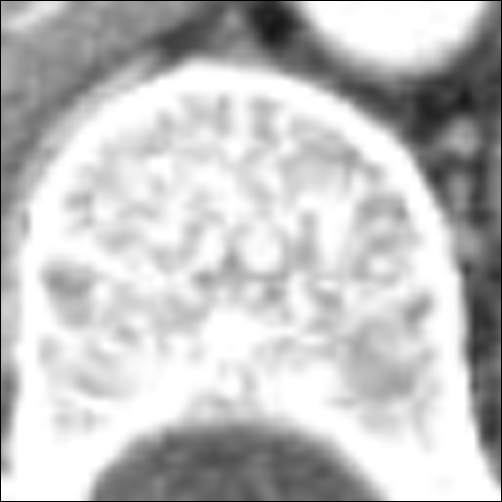
\includegraphics[width=3.6cm]{./img/bicubic.png} \label{interpolation:bicubic}}
}
\caption{Vergleich der Nearest Neighbor, bilinearen und bikubischen Interpolation}
\label{interpolation}
\end{figure*}

Bei der bilinearen Interpolation werden die zu der Koordinate $(x_0, y_0)$ nächstliegenden vier Werte der Bildpunkte des Originalbildes zur Interpolation verwendet\cite[S.387]{burger:bv}. In Abbildung \ref{bilinear_interpolation} sind das \textit{A}, \textit{B}, \textit{C} und \textit{D}. Zuerst findet eine Interpolation in x-Richtung statt. Daraus ergeben sich die Werte \textit{E} und \textit{F}. Durch die Interpolation in y-Richtung der Werte \textit{E} und \textit{F} wird der finale Wert \textit{G} ermittelt.

\begin{figure}[htbp]
  \vspace{0.5cm}
  \centering
  \fbox{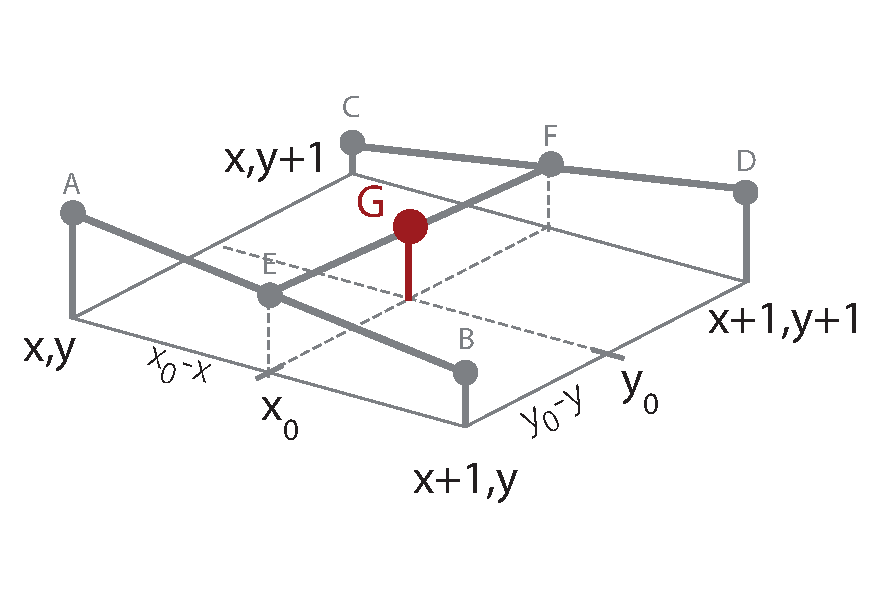
\includegraphics[angle=0,width=10cm]{./img/bilinear_interpolation.pdf}}
   \caption{Bilineare Interpolation \cite[S.388]{burger:bv}}
  \label{bilinear_interpolation}
  \vspace{0.5cm}
\end{figure}

Für jeden Bildpunkt des Zielbildes \textit{Z} wird der Referenzpunkt im Originalbild \textit{S} mittels einer Normalisierung gefunden.

\begin{equation}
 x_{0} = \frac{x_{Z}}{width_{Z}}\cdot width_{S}\qquad
 y_{0} = \frac{y_{Z}}{height_{Z}}\cdot height_{S}
\end{equation}

Zu den Werten von $x_{0}$ und $y_{0}$ müssen nach Burger und Burge\cite[S. 387 ff]{burger:bv} die nächstliegenden Bildwerte ermittelt werden.

\begin{equation}
A= S(x,y) \qquad B=S(x+1,y) \qquad C=S(x,y+1)\qquad D=S(x+1,y+1)
\end{equation}

wobei $x$ und $y$ die abgerundeten Werte von $x_{0}$ und $y_{0}$ darstellen. Die Werte \textit{E} und \textit{F} werden durch den Abstand von $x_{0}$ und $x$ ermittelt.

\begin{equation}
E = A + (x_0 - x) \cdot (B - A)
\end{equation}
\begin{equation}
F = C + (x_0 - x) \cdot (D-C)
\end{equation}

Nach der horizontalen Interpolation wird der finale Wert \textit{G} aus dem Abstand von $y_0$ und $y$ berechnet.

\begin{equation}
G = E + (y_0 - y) \cdot (F-E)
\end{equation}

Der Wert von \textit{G} kann nun beim Zielbild \textit{Z} an die aktuelle Position gesetzt werden. Bei Farbbildern wird jeder Kanal separat interpoliert.

\subsection{Anzeige der Zusatzinformationen}

Dem Benutzer werden direkt auf der Zeichenfläche wichtige Zusatzinformationen angezeigt. So kann der Anwender die aktuelle Größe des Bildes in Pixeln und das prozentuale Verhältnis zum Originalbild ablesen, sowie die gewählten Fensterungswerte einsehen. Neben den Bildeigenschaften werden auch dynamische Inhalte angezeigt wie das Patientenkoordinatensystem und Orientierungslinien. Orientierungslinien markieren in gleichen geöffneten 3D-Datensätzen mit unterschiedlicher Ebenenansicht einen gemeinsamen Punkt. Diese dynamischen Aspekte werden folgend erläutert.

\subsubsection{Das Koordinatensystem}

Der DICOM-Standard definiert ein sogenanntes \textit{Reference Coordinate System} \cite[S. 55]{dicom:iod} und dient zur Orientierung des Patienten im Raum. Es werden sechs Richtungen der drei Achsen definiert, womit die Lage des Patienten beschrieben werden kann \cite[C.7.6.1.1.1]{dicom:iod}. 

\begin{itemize}
\item \textbf{R} (right) - \textbf{L} (left) - \textbf{x} \\
	Right bestimmt die rechte, left die linke Hand des Patienten.
\item \textbf{A} (anterior) - \textbf{P} (posterior) - \textbf{y} \\
   Die Vorderseite des Patienten wird als Anterior, die Rückseite als Posterior bezeichnet.
\item \textbf{F} (foot) - \textbf{H} (head) - \textbf{z} \\
 Foot steht für den Patientenfuß und Head für den Kopf.
\end{itemize}

\begin{figure*}[htb]
%\subfigure[Keypoints]{\includegraphics[width=0.49\textwidth]{./img/basmati_keypoints.png}}\hfill
\centering
\fbox{
\subfigure[Die x- und z-Achse]{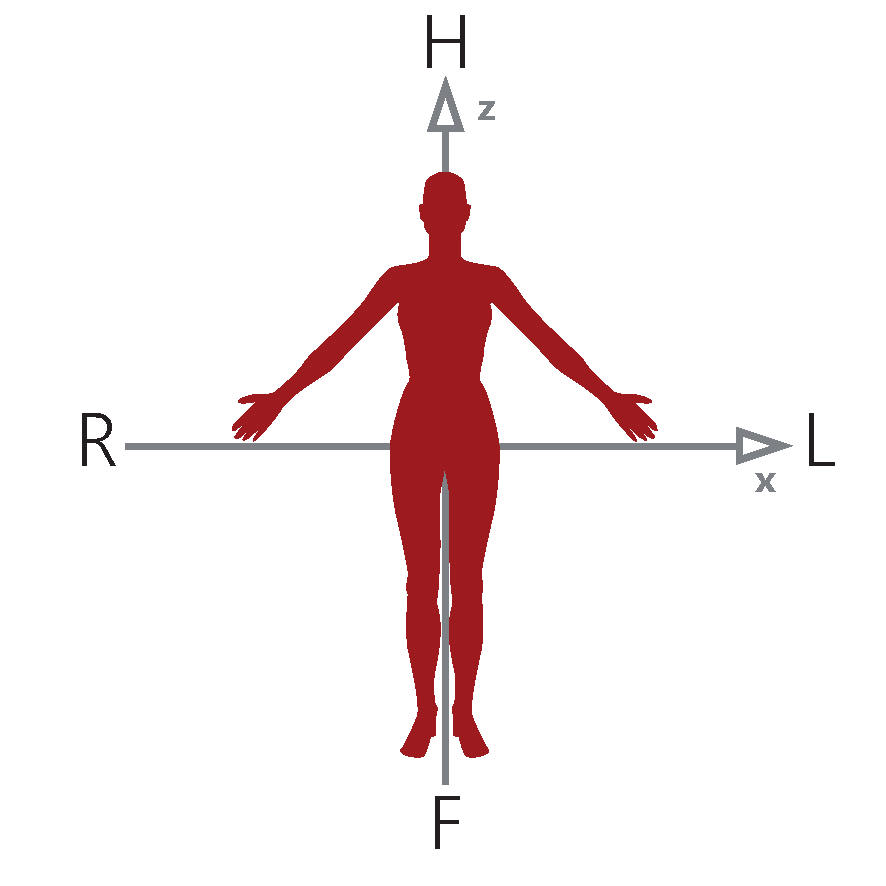
\includegraphics[width=7cm]{./img/coords1.pdf} \label{coords:xz}}
\subfigure[Die y- und z-Achse]{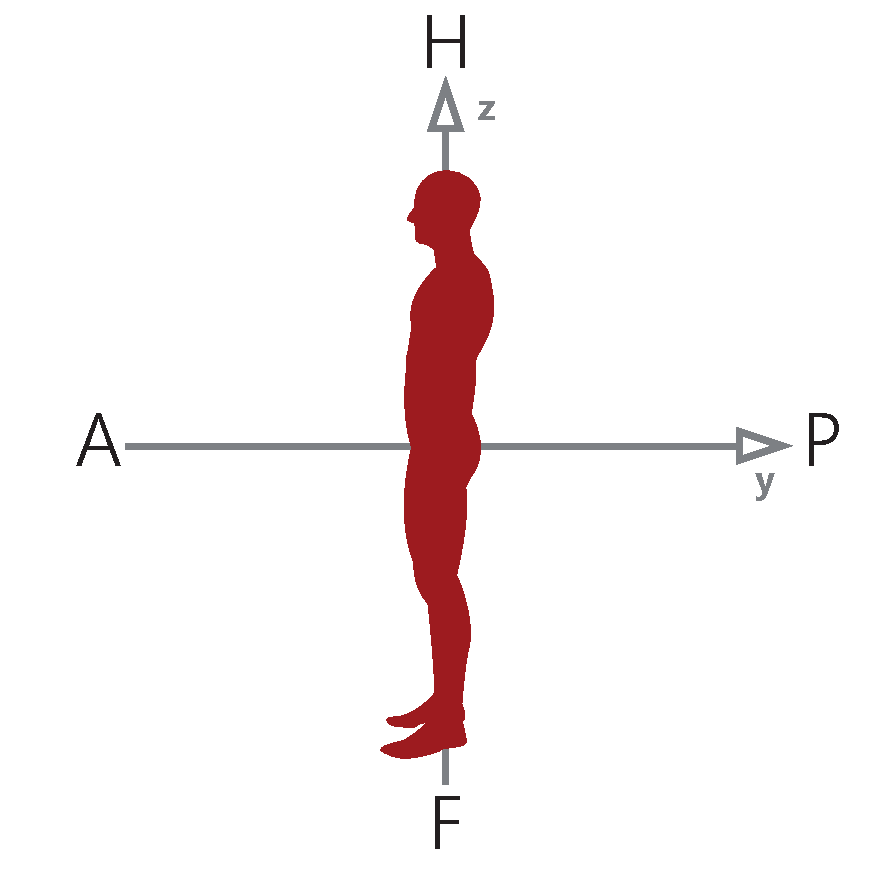
\includegraphics[width=7cm]{./img/coords2.pdf} \label{coords:yz}}
}
\caption{Das patientenbasierte Koordinatensystem}
\label{coords:both}
\end{figure*}

Wie in Abbildung \ref{coords:xz} dargestellt, steigt die x-Achse in Richtung der linken Hand das Patienten. Die Werte der y-Achse nehmen von der Vorderseite zur Rückseite des Patienten zu. Die z-Achse erhöht sich in Richtung der Füße zum Kopf des Patienten\cite[C.7.6.2.1.1]{dicom:iod}.\\
Unter Berücksichtigung des DICOM-Tags \textit{Image Orientation} mit dessen Vektoren kann die Beschriftung der Koordinatenachsen bestimmt werden. Durch den maximalen Betrag der Elemente der Vektoren wird die dominanten Achsen ermittelt. Dadurch erhält man die Koordinatenachsen der Bildebene. Des weiteren kann durch die Achsen die Ebenendarstellung bestimmt werden. Ein dominanter xy-Anteil bedeutet \textit{axiale} Ebenendarstellung, der xz-Anteil ist die \textit{coronale} Ansicht und der yz-Anteil die \textit{sagittale} Darstellung.

\begin{equation}
\vec{r}=\left(\begin{array}{c} 1 \\ 0 \\ 0 \end{array}\right) \qquad
\vec{c}=\left(\begin{array}{c} 0 \\ 1 \\ 0 \end{array}\right)
\vspace{0.5cm}
\label{orientationvecs}
\end{equation}

Beispiel \ref{orientationvecs} zeigt zwei Vektoren von \textit{ImageOrientation}. Die dominanten Achsen sind das x-Element aus $\vec{r}$ mit dem Wert $1$ und das y-Element aus $\vec{c}$ ebenfalls mit $1$. Durch den dominanten Anteil können die Achsen abgelesen werden, die auf die Bildebene gezeichnet werden. Die x-Achse bekommt auf der negativen Seite \textit{R} und \textit{L} auf der positiven Seite. Die zweite Achse der Bildebene ist y mit der negativen Seite \textit{A} und positiver Seite \textit{P}. Die z-Achse mit \textit{H} und \textit{F} ragt aus der Bildebene heraus beziehungsweise hinein. Sind die Elemente negativ ist die Richtung der Koordinatenachsen vertauscht. Aus den Beispielvektoren ergibt sich folgende Darstellung der Achsen wie in Abbildung \ref{axialbsp} dargestellt.

\begin{figure}[htbp]
  \vspace{0.5cm}
  \centering
  \fbox{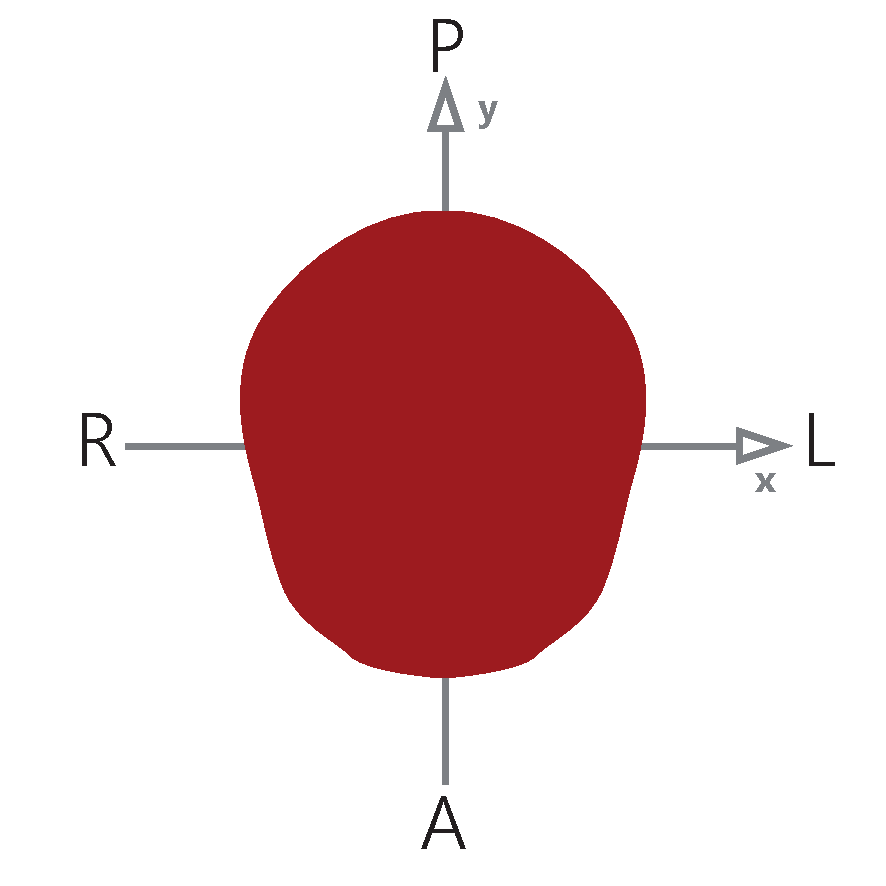
\includegraphics[angle=0,width=6cm]{./img/axialbsp.pdf}}
   \caption{Beschriftung der Koordinatenachsen bei axialer Ebenendarstellung}
  \label{axialbsp}
  \vspace{0.5cm}
\end{figure}

\subsubsection{Zeichnen der Orientierungslinien}\label{scoutinglines}

Wenn mehrerer gleiche Datensätze in unterschiedlichen Ebenendarstellungen geöffnet sind, helfen dem Anwender die Orientierungslinien bei der Navigation durch den dreidimensionalen Datensatz. Abbildung \ref{lines:single:a} zeigt eine axiale Ebenedarstellung als aktuelle Anzeige, die vom Benutzer bedient wird. Zusätzlich sind die coronale (Abbildung \ref{lines:c}) und sagittale Ansicht (Abbildung \ref{lines:s}) geöffnet. Da der Anwender in der axialen Ansicht arbeitet, werden Änderungen der Bildanzeige an die beiden Beobachter weitergegeben.\\
Navigiert der Nutzer mit der Scrollleiste durch den axialen Datensatz, wird mit Hilfe des Oberserver-Musters bei jeder Änderung die aktuelle z-Koordinate der Bildschicht an die coronale und sagittale Darstellung übertragen. Dieser z-Wert wird an der entsprechenden Stelle der Bildschicht als, im Beispiel blaue, Orientierungslinie eingezeichnet. \\
Wie in den Abbildungen \ref{lines:single} zu sehen ist, entspricht die z-Koordinate in axialer Ansicht der y-Koordinate der coronalen und sagittalen Darstellung. Daraus folgt, dass die Orientierungslinie an der Stelle von $(0, y_{coronal}) $ bis $(width, y_{coronal})$ sowie von $(0, y_{sagittal}) $ bis $(width, y_{sagittal})$ für $y_{coronal}, y_{sagittal} = z_{axial}$

\begin{figure*}[htb]
%\subfigure[Keypoints]{\includegraphics[width=0.49\textwidth]{./img/basmati_keypoints.png}}\hfill
\centering
\fbox{
\subfigure[Axiale Ebenendarstellung]{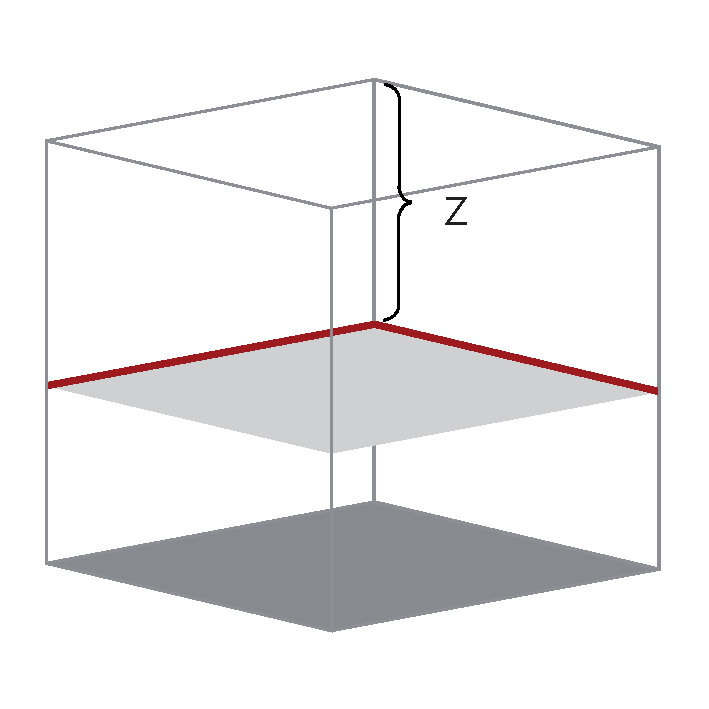
\includegraphics[width=5cm]{./img/lines_axial_single.pdf} \label{lines:single:a}}
\subfigure[Orientierungslinie der axialen Darstellung in der coronalen Ebenendarstellung]{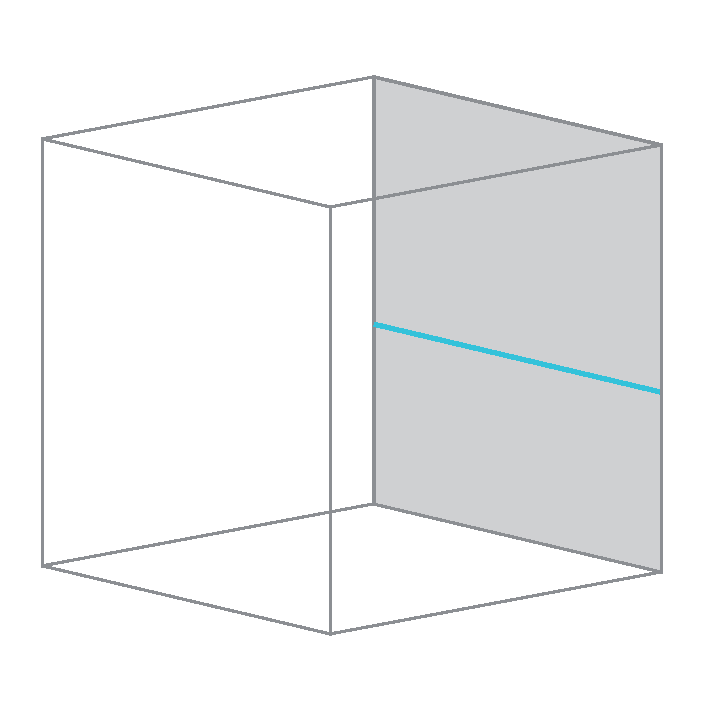
\includegraphics[width=5cm]{./img/lines_coronal_single.pdf} \label{lines:single:c}}
\subfigure[Orientierungslinie der axialen Darstellung in der sagittalen Ebenendarstellung]{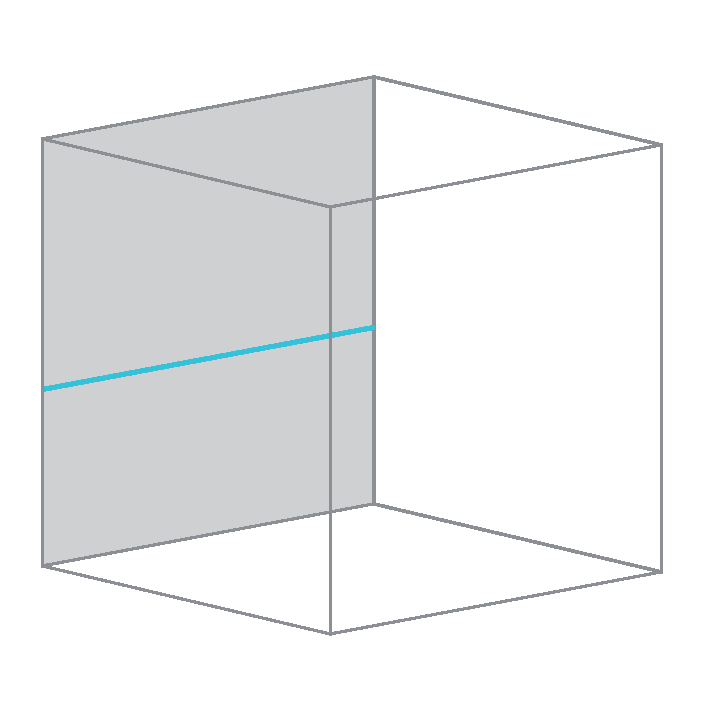
\includegraphics[width=5cm]{./img/lines_sagittal_single.pdf} \label{lines:single:s}}
}
\caption{Einfache Darstellung der Orientierungslinien}
\label{lines:single}
\end{figure*}

Die Koordinaten zum Einzeichnen der Orientierungslinien sind abhängig von der Quell- und Zieldarstellung. Navigiert der Anwender in der sagittalen Ebenendarstellung und aktualisiert damit eine axiale Anzeige entspricht die Koordinate $z_{sagittal}  = x_{axial}$. Die Orientierungslinie wird damit durch die Punkte $(x_{axial}, 0) $ und $(x_{axial}, height)$ definiert. Diese Vorgehensweise wird bei einer Navigation mit der Scrollleiste umgesetzt. Eine weitere Möglichkeit zur Orientierung im Datensatz ist die direkte Auswahl eines Punktes.

\begin{figure*}[htb]
%\subfigure[Keypoints]{\includegraphics[width=0.49\textwidth]{./img/basmati_keypoints.png}}\hfill
\centering
\fbox{
\subfigure[Punktauswahl in axialer Ebenendarstellung]{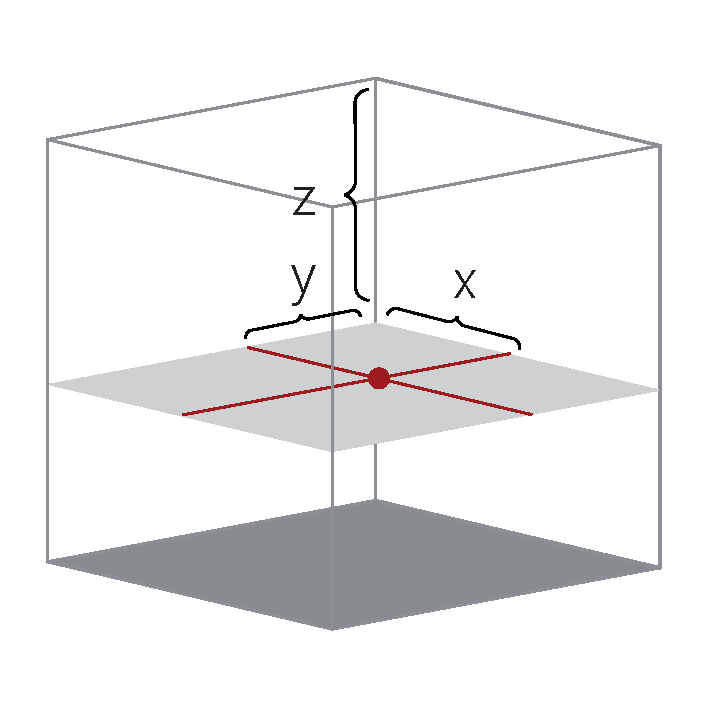
\includegraphics[width=5cm]{./img/lines_axial.pdf} \label{lines:a}}
\subfigure[Anzeige des referenzierten Punktes aus der axialen Darstellung in der coronalen Ebene]{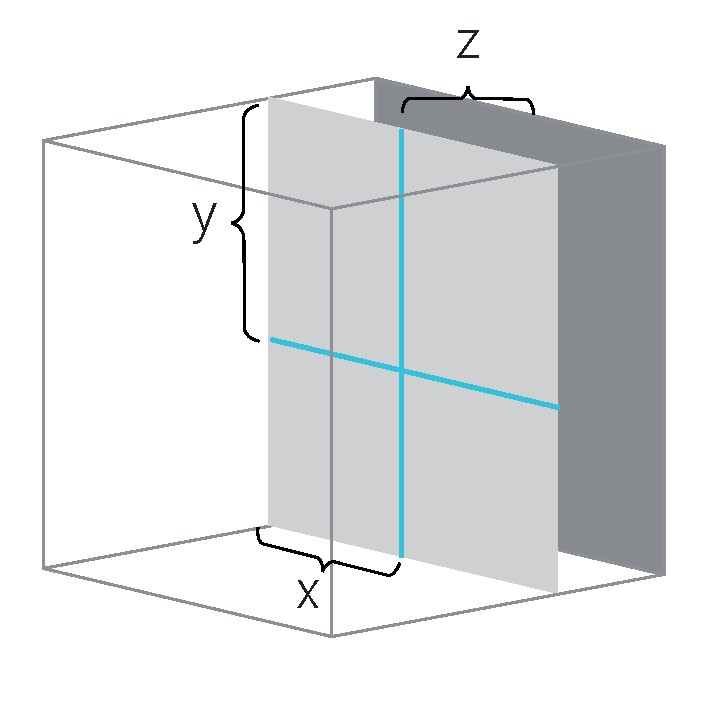
\includegraphics[width=5cm]{./img/lines_coronal.pdf} \label{lines:c}}
\subfigure[Anzeige des referenzierten Punktes aus der axialen Darstellung in der sagittalen Ebene]{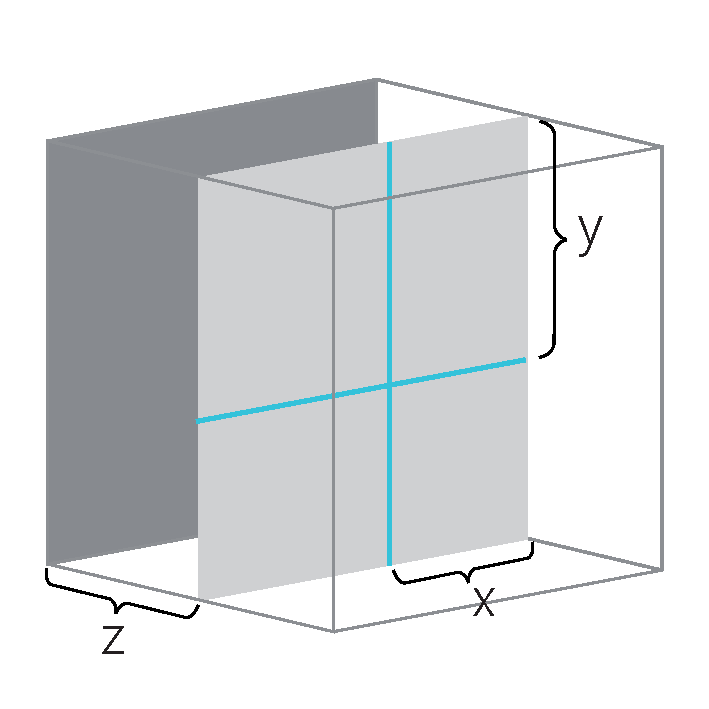
\includegraphics[width=5cm]{./img/lines_sagittal.pdf} \label{lines:s}}
}
\caption{Anzeige eines referenzierten Punktes in axialer Ebene mit Hilfe der Orientierungslinien}
\label{lines}
\end{figure*}

Abbildung \ref{lines:a} zeigt einen vom Anwender gewählten Punkt in der axialen Darstellung. Wieder müssen alle Beobachter, also Bildanzeigen mit dem gleichen Datensatz, nach der Auswahl aktualisiert werden. Die Abbildungen \ref{lines:single} zeigen nur die aktuell vom Nutzer gewählte Bildschicht der aktiven Anzeige. Bei einer direkten Punktauswahl wird in allen Ansichten der gleiche Punkt im Raum $(x, y, z)$ referenziert. Das bedeutet, es werden sowohl die horizontale, als auch die vertikale Orientierungslinie eingezeichnet. Zusätzlich wird die angezeigte Bildschicht der Beobachter den Koordinaten angepasst. Der gewählte Punkt wird jeweils durch den Schnittpunkt der Orientierungslinien symbolisiert. Das Beispiel der Abbildungen in \ref{lines} zeigt eine aktive axiale Ansicht sowie eine coronale und sagittale Ebenendarstellung als Beobachter.\\
Der vom Anwender gewählte Punkt im Raum ist:

\begin{equation}
P_{axial}=\left(\begin{array}{c} x_{axial} \\ y_{axial} \\ z_{axial} \end{array}\right) 
\vspace{0.5cm}
\end{equation}
Aus diesem Punkt müssen die Koordinaten für die Orientierungslinien und der Bildschicht bestimmt werden.
Für die Darstellung von der axialen Ansicht zum referenzierten coronalen Punkt folgt aus Abbildung \ref{lines:c}:
\begin{equation}
P_{coronal}=\left(\begin{array}{c} x_{coronal} \\ y_{coronal} \\ z_{coronal} \end{array}\right) =
\left(\begin{array}{c} x_{axial} \\ z_{axial} \\ y_{axial} \end{array}\right)
\vspace{0.5cm}
\end{equation}

Mit diesen Koordinaten ergeben sich für die coronale Ebenendarstellung die vertikale Orientierungslinie von $(x_{axial}, 0)$ bis $(x_{axial}, height)$, die horizontale Linie $(0, z_{axial})$ bis $(width, z_{axial})$ und der Index der Bildschicht $y_{axial}$.\\
Auch dieses Vorgehen ist abhängig von der Quell- und Zieldarstellung der aktiven Darstellung und Beobachtern.

\subsection{Implementierung der Werkzeuge}

Die Anzeige der Orientierungslinien komplettiert die Funktionalitäten zur Bilddarstellung, Navigation und Orientierung. Der nächste Schritt befasst sich mit der Manipulation der Bilddaten mit den zur Verfügung gestellten Werkzeugen.\\
Die Werkzeuge bilden die Schnittstelle zwischen Anwender und dem System. So werden Benutzereingaben entgegengenommen, interpretiert und auf der Zeichenfläche umgesetzt. Das \textit{DicomCanvas} reagiert mit Hilfe verschiedener \textit{Listener} auf die eintretenden Ereignisse, wie beispielsweise einem Mausklick oder Tastendruck. Diese Ereignisse, auch \textit{Events} genannt, werden an das Werkzeug weitergeleitet, damit das Bild und die Zeichenfläche manipuliert werden kann. Das Canvas ruft die Werkzeuge bei gängigen Maus-Events auf, die in der folgenden Liste genauer dargestellt werden.

\begin{itemize}
\item \textbf{MouseEnter} \\
	Dieses Event wird ausgelöst, wenn der Mauszeiger die Zeichenfläche betritt.
\item \textbf{MouseExit} \\
	Das Ereignis ist das Gegenstück zu MouseEnter. Beim Verlassen tritt dieses Event ein.
\item \textbf{MouseMove} \\
	Solange sich der Mauszeiger auf der Zeichenfläche befindet und in Bewegung ist, wird das Werkzeug mit den aktuellen Koordinaten des Cursors aktualsiert.
\item \textbf{MouseDown} \\
	Dieses Ereignis tritt ein, wenn der Mauszeiger gedrückt wird und sich über der Zeichenfläche befindet. Zusätzlich wird im Werkzeug hinterlegt, dass eine Maustaste\footnote{Das Event wird unabhängig von der Nummer der gedrückten Maustaste ausgelöst. Innerhalb der Funktion, die das Ereignis abfängt, kann ausgelesen werden, ob die erste, zweiter oder dritte Maustaste betätigt wurde.} gedrückt wurde.
\item \textbf{MouseUp} \\
	Wird die Maustaste nach dem Drücken losgelassen, tritt das MouseUp-Ereignis ein. Dies wird innerhalb des Werkzeugs übernommen.
\item \textbf{MouseWheel} \\
	Beim Bewegen des Mausrads wird unabhängig von der Richtung das MouseWheel-Event ausgelöst\footnote{Die Drehrichtung kann, wie bei den Mausklicks, innerhalb der abfangenden Funktion ausgelesen werden}.
\end{itemize}

Zusätzlich zu den Ereignissen definieren Werkzeuge noch zwei Einhängepunkte (Hooks), die in den Zeichenprozess eingebunden werden. Wie in Abschnitt \ref{drawandmanipulate} in Abbildung \ref{imageprocess} dargestellt, werden diese Hooks vor der Berechnung der Bildkoordinaten und nach dem Zeichenprozess der Zusatzinformationen aufgerufen. Die Einhängepunkte bieten den Werkzeugen die Möglichkeit, etwas zu dem Zeichenprozess beizutragen, falls diese Funktion gewünscht ist. So kann beispielsweise ein Fenster am Mauszeiger gezeichnet werden, das aktuelle Informationen über Pixelwerte darstellt.\\
Damit die Zeichenfläche gelesen und bearbeitet werden kann, steht jedem Werkzeug das zugehörige \textit{DicomCanvas} als Datenelement zur Verfügung. Dadurch können zum Beispiel die Daten der Zeichenfläche oder Bildinformationen ausgelesen werden. Dazu zählen unter anderem der Bildstapel sowie die aktuelle Bildschicht und die Koordinaten auf der Zeichenfläche. Die abstrakte Klasse der Werkzeuge \textit{ATool} liefert dem Entwickler die Informationen zum Mauszeiger und dessen Eigenschaften. Dazu zählen die aktuelle x- und y-Position des Cursors auf der Zeichenfläche und ob ein Button der Maus gedrückt ist. Wird eine der Maustasten betätigt, wird eine Startpunkt erstellt. Nach dem Loslassen des Buttons wird der Endpunkt gespeichert, womit Start und Ende die Strecke der Maus von zwei Punkten nach dem Drücken bis zum Loslassen darstellen.\\
Aus diesen verfügbaren Informationen lassen sich vielfältige Werkzeuge erzeugen. 

\subsubsection{Das Bild bewegen mit dem MoveTool}
Mit Hilfe des \textit{MoveTools} lässt sich die aktuelle Bildschicht über die Zeichenfläche schieben. Beim ersten Klick innerhalb des \textit{DicomCanvas} speichert das Werkzeug die Cursorposition als Startpunkt. Solange die Maustaste gedrückt bleibt, wird der neue Mittelpunkt des Bildes aus der aktuellen Mauszeigerposition bestimmt. Die Berechnung erfolgt mit dem Verbindungsvektor aus Startpunkt S und dem Endpunkt E mit 
\begin{equation}
\overrightarrow{SE}=\left(\begin{array}{c} E_x - S_x \\ E_y  - S_y\\ \end{array}\right)
\vspace{0.5cm}
\end{equation}

Die direkte Berechnung von $\overrightarrow{SE}$ ist aufgrund mehrerer aufeinanderfolgender Zeichenzyklen nicht möglich. Abbildung \ref{movetool} zeigt diese Zyklen durch die roten Pfeile. Bei jeder Mausbewegung wird die Zeichenfläche neu gezeichnet. 

\begin{figure}[htbp]
  \vspace{0.5cm}
  \centering
  \fbox{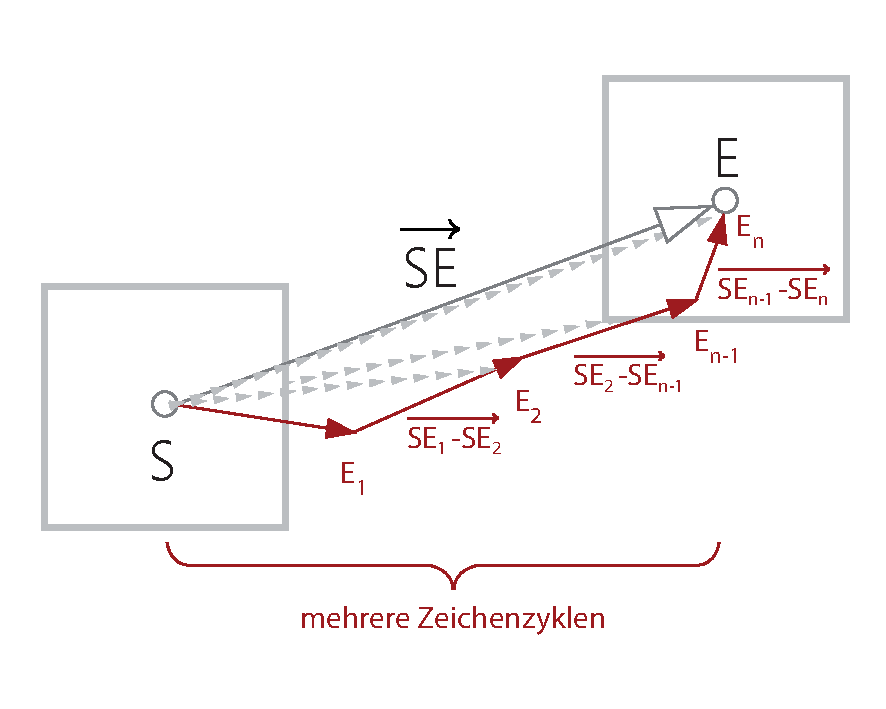
\includegraphics[angle=0,width=8cm]{./img/movetool.pdf}}
   \caption{Translation des Bildmittelpunkts}
  \label{movetool}
  \vspace{0.5cm}
\end{figure}

Nach der ersten Translation befindet sich der Bildmittelpunkt an der Stelle $S + \overrightarrow{SE_1}$, in der folgenden an $S + \overrightarrow{SE_2}$ bis die Maus an $E_n$ losgelassen wird und der neue Bildmittelpunkt $S + \overrightarrow{SE_n}$ ist (Dargestellt durch die gestrichelten Linien). Da bei jeder Translation ein neuer Bildmittelpunkt bestimmt wird, erfolgt die richtige Berechnung aus der Differenz zwischen der vorherigen und der aktuellen Transformation. Durch Addition von Bildmittelpunkt und der Differenz erhält man das richtig translierte aktuelle Bildzentrum.

\begin{equation}
E_n= E_{n-1} + (\overrightarrow{SE_{n-1}}-\overrightarrow{SE_n})
\vspace{0.5cm}
\end{equation}

$E_n$ ist der zu bestimmende Bildmittelpunkt für die Translation. Das aktuelle Zentrum ist $E_{n-1}$. Die zuletzt durchgeführte Verschiebung ist $\overrightarrow{SE_{n-1}}$, während die aktuelle durch $\overrightarrow{SE_n}$ dargestellt ist.

\subsubsection{Skalierung mit dem ResizeTool}

Das \textit{ResizeTool} ermöglicht dem Anwender das Bild zu verkleinern oder zu vergrößern. Durch das Zoomen können Details auch in kleinen Bildgrößen genauer betrachtet werden\footnote{Das vergrößerte Bild ist nur eine Interpolation der originalen Pixelwerte}.\\
Ein Mausklick in die Zeichenfläche löst den Skalierungsprozess aus. Das Werkzeug reagiert speziell auf das \textit{MouseMove} Ereignis. Die Bewegung in y-Richtung auf der Zeichenfläche bestimmt den Skalierungsfaktor. Der Faktor wird folgendermaßen berechnet, wobei $S_y$ dem y-Wert des Startpunktes  und $E_y$ dem y-Wert des Endpunktes entspricht: 

\begin{equation}
scale = \frac{S_y - E_y}{100}
\vspace{0.5cm}
\end{equation}

Ein Endpunkt in positiver Richtung\footnote{Da der Ursprung der Zeichenfläche in der oberen linken Ecke liegt, ist die positive y-Richtung die untere Kante des Canvas} vergrößert das Bild, während die ein Ziehen der Maus in die negative Richtung das Bild verkleinert. Mit einer Division durch $100$ entsprechen $10$ Pixel ein positiver oder negativer Richtung eine Größenänderung von $10\%$. Bei einem Verhältnis von $1:1$ lässt sich die Skalierung nicht mehr kontrollieren, da die Größe rasch zu- beziehungsweise abnimmt.\\
Ähnlich dem \textit{MoveTool} muss vor der Skalierung der alte Faktor abgezogen werden, damit in gleichem Verhältnis skaliert wird.

\subsubsection{Das DefaultTool}

Das \textit{DefaultTool} stellt ein besonderes Werkzeug dar, da es selbst keine Funktionalitäten implementiert. Es nutzt die Funktionen des \textit{MoveTools} und des \textit{ResizeTools}. Im \textit{DefaultTool} wird geprüft, welche Maustaste gedrückt wird. Bei einem Linksklick wird das \textit{MoveTool} und der Translationsprozess ausgeführt. Ein Klick mit der rechten Maustaste in das Bild nimmt die Koordinaten des Cursors auf, um darauf alle weiteren Zeichenflächen, die Beobachter, zu informieren, dass ein Punkt gewählt wurde. Darauf aktualisieren die Beobachter Bildschicht und Orientierungslinien wie in Abschnitt \ref{scoutinglines} beschrieben. Das \textit{ResizeTool} wird durch das Drehen des Mausrads angestoßen und bewirkt pro Einheit eine Größenänderung von $10\%$.

\subsubsection{Justierung der Fensterung mit dem WindowTool}

Eine Einstellung der Fensterungswerte kann mit dem \textit{WindowTool} vorgenommen werden. Das Werkzeug arbeitet sowohl in der x-, als auch y-Richtung. Wird der Cursor auf der x-Achse bewegt, kann der Wert des Zentrums (\textit{WindowCenter}) angepasst werden. Die Fensterungsbreite (\textit{WindowWidth}) wird über die y-Achse eingestellt. Der Wert um wie viel \textit{WindowWidth} und \textit{WindowCenter} erhöht werden, wird mit dem Startpunkt $S$ und Endpunkt $E$ bestimmt. $\overrightarrow{SE}$ wird darauf auf die bestehenden Werte des Zentrums und der Fensterungsbreite addiert.

\subsubsection{Punktauswahl mit dem PointTool}

Das Werkzeug \textit{PointTool} erfüllt zwei Aufgaben. Zum einen gibt es die Möglichkeit einzelne Punkte zu markieren und im Bild zu hinterlegen, zum anderen können zu den Pixeln mit Hilfe eines Tooltips\footnote{Tooltips sind kleine Fenster, die an der Stelle des Cursors Informationen einblenden} zusätzliche Informationen angezeigt werden. Dazu zählen die Koordinaten des Pixels, der tatsächliche Wert und der mit Hilfe der Fensterung interpolierte Wert. Aus der aktuellen Position und den Bildkoordinaten kann bestimmt werden, ob der Cursor innerhalb des Bildes liegt. Liegt der Mauszeiger im Bild können Punkte gewählt und Informationen zu den Pixelwerten ausgegeben werden.
\begin{itemize}
\item \textbf{Punktauswahl}\\
	Ein Punkt wird gewählt nachdem eine Maustaste betätigt und wieder gelöst wird. Liegt der Punkt innerhalb des Bildes, erfolgt eine Umrechnung in normalisierte Koordinaten im Intervall $[0,1]$ und wird dem Bild hinzugefügt.
\item \textbf{Ausgabe der Information}\\
	Das Anzeigen eines Tooltips ist ein Beispiel eines Einhängepunktes(Hook) für Werkzeuge. Ist der Zeichenprozess beendet, sollen die zusätzlichen Informationen auf die Zeichenfläche gemalt werden.
	Dazu wird an der Position des Cursors ein Rechteckt mit den Pixeldaten gezeichnet.
\end{itemize}

\section{Dynamische Parametervergabe}

Mit dem Punktauswahlwerkzeug erhält der Benutzer die Möglichkeit, dynamisch spezifische Bildpunkte zu wählen. Die Selektion kann anschießend innerhalb eines Plug-ins ausgelesen werden. So können zum Beispiel Start- oder Saatpunkte für Algorithmen gesetzt werden. Als weiteren dynamischen Aspekt soll der Benutzer vor dem Ausführen eines Plug-ins selbst Parameter bestimmen können. So können beispielsweise Schwellwerte im Bezug zu speziellen Pixelwerten gewählt werden. Die dynamischen Parameter bestehen allerdings nicht immer aus numerischen Werten. So müssen ebenso Zeichenketten oder Dateien übergeben werden können. Durch die Dateiauswahl können beispielsweise Textdateien ausgewählt werden, die für ein Plug-in benötigte Datensätze enthalten. Des Weiteren besteht die Möglichkeit DICOM-Dateien zu laden, um unabhängige DICOM-Objekte innerhalb des Plug-ins als Referenzbilder zu erzeugen.\\
Mit dem generischen Dialogfenster aus Abschnitt \ref{genericdialog} soll der Benutzer die Möglichkeit erhalten Parametertypen nach Wahl zusammenzustellen. Hierzu stellt die Klasse \textit{GenericPlugInDialog} verschiedene Typen zur Verfügung.

\begin{itemize}
\item \textbf{Checkbox}\\
Die Checkbox wird verwendet wenn ein bool'scher Parametertyp gewünscht wird. Markiert symbolisiert die Box den Wert \textit{true}, ansonsten \textit{false}.
\begin{figure}[H]
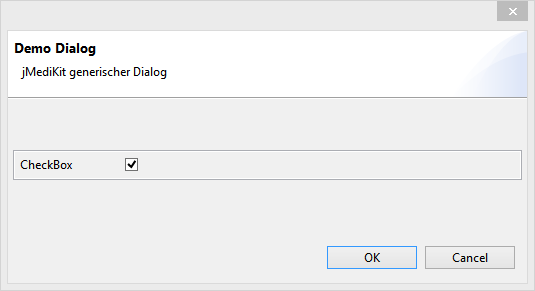
\includegraphics[angle=0,width=6cm]{./img/checkbox.png}
\end{figure}

\item \textbf{RadioGroup}\\
Mit Hilfe der Radio Group kann ein bestimmter Wert aus einer Gruppe gewählt werden. Der Parametertyp gibt jeweils die Selektion als Zeichenkette zurück.
\begin{figure}[H]
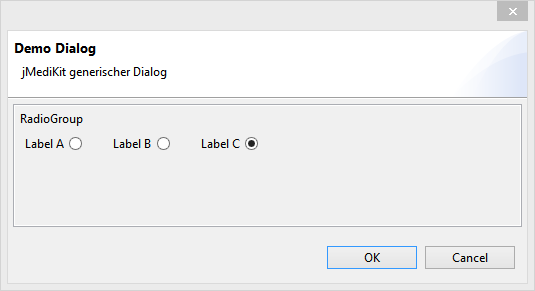
\includegraphics[angle=0,width=6cm]{./img/radiogroup.png}
\end{figure}

\item \textbf{FileDialog}\\
Mit dem FileDialog kann der Anwender eine Datei in das Plug-in laden. Wird der Parameter ausgelesen, wird der Pfad als Zeichenkette zurückgegeben.
\begin{figure}[H]
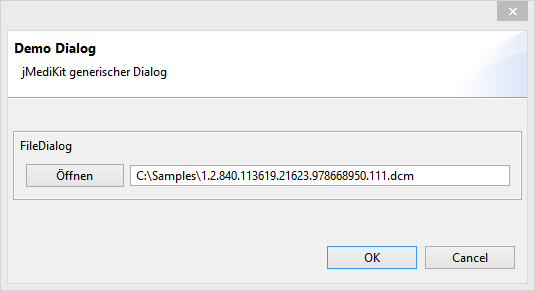
\includegraphics[angle=0,width=6cm]{./img/filedialog.png}
\end{figure}

\item \textbf{Slider}\\
Der Slider definiert ein Intervall $[x,y]$ aus dem ein Wert gewählt werden kann. Dieser Parametertyp wird eingesetzt, wenn untere und obere Wertgrenzen existieren oder die Benutzereingabe begrenzt werden soll. Der Wert wird als Fließkommazahl zurückgegeben.
\begin{figure}[H]
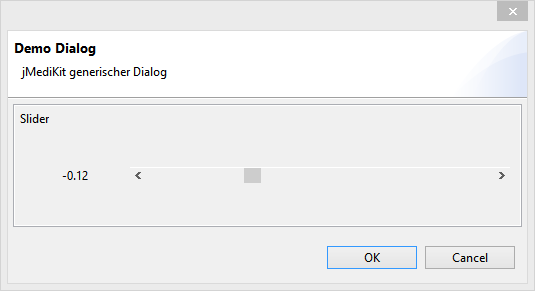
\includegraphics[angle=0,width=6cm]{./img/slider.png}
\end{figure}

\item \textbf{StringItem, IntegerItem, FloatItem}\\
Diese drei Parametertypen verhalten sich ähnlich. Sie nehmen den jeweiligen Wert des entsprechenden Typs entgegen und geben diesen beim Auslesen wieder zurück.
\begin{figure}[H]
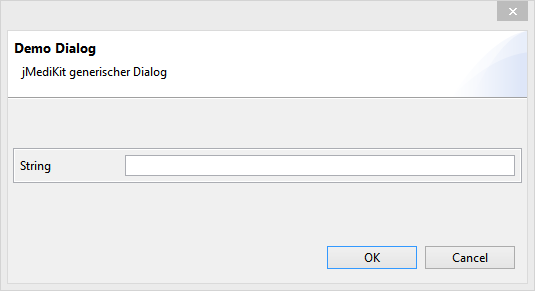
\includegraphics[angle=0,width=6cm]{./img/stringitem.png}
\end{figure}

\end{itemize}

Die unterschiedlichen Parametertypen können beliebig miteinander in einem einzigen Dialog kombiniert werden.

\section{Debugging der eigenen Plug-ins}

Das Java Medical Imaging Toolkit bietet sowohl eine dateibasierte, als auch eine visuelle Ausgabeart um das Debugging zu erleichtern und eventuelles Fehlverhalten der Plug-ins zu finden.

\subsection{Dateibasiertes Debugging}
Debugging hilft dem Benutzer Variablen zu überprüfen oder Programmabläufe zu verstehen. Da ein umfassendes Debugsystem nicht verfügbar ist, muss die Fehlersuche über Programmausgaben erfolgen. Die Standardausgabe nicht im Rich Client nicht einsehbar ist, wird mit Dateien gearbeitet, die Ausgaben protokollieren.\\
In der Klasse \textit{APlugIn} ist eine Methode \textit{setOutput} definiert. Da sowohl \textit{APlugIn2D} als auch \textit{APlugIn3D} von dieser Klasse erben, ist die Methode in allen Plug-ins verfügbar. Wird diese zum Beispiel in den Optionen einen Plug-ins aufgerufen, wird die Standardausgabge \textit{out} von \textit{java.lang.System} auf die als Parameter spezifizierte Datei umgeleitet. Dadurch werden alle Aufrufe von \textit{System.out.println} in dieser Datei abgelegt.

\subsection{Visuelles Debugging}
In manchen Situationen ist es nützlich, spezielle Zwischenschritte der Algorithmen ausgeben zu lassen. Manche Bildverarbeitungsprozesse erwarten zum Beispiel ein vorgefiltertes Bild oder ein spezielles Bildformat wie ein Binärbild. Das visuelle Debugging erlaubt die Kontrolle dieser Zwischenschritte durch eine unabhängige Bildausgabe.\\
Um diese Problematik zu lösen, ist im jMediKit die Klasse \textit{Visualizer} vorhanden. Die statische Methode \textit{show} nimmt entweder ein Bild oder eine Liste von Bildern entgegen. Wird diese aufgerufen, werden die übergebenen Bilder in einem separaten Fenster angezeigt.

